\documentclass[12pt,a4paper]{report}
\usepackage[top=2.5cm,bottom=2.5cm,left=1.5cm,right=1.5cm]{geometry}

\usepackage{cmap}
\usepackage{graphicx}
\usepackage[english,slovak]{babel}
\usepackage[utf8]{inputenc}
\usepackage[T1]{fontenc}
%\usepackage{lmodern}

\usepackage{amssymb}
\usepackage{amsmath}

\usepackage{amsthm}
\newtheorem{veta}{Veta}[section]
\newtheorem{lema}[veta]{Lema}
\theoremstyle{definition}
\newtheorem{definicia}{Definícia}[chapter]
\theoremstyle{remark}
\newtheorem*{poznamka}{Poznámka}

\usepackage{setspace}
\usepackage{caption}
\usepackage{grffile}
\usepackage{float}
\onehalfspacing

\begin{document}

%\includepdf{zadanie.pdf}

%%% DEFINÍCIE NÁZVOV
\def\nazov{Záverčná správa}
\def\autorJ{Jaroslav Fúska }
\def\autorT{Tomáš Sláma }
\def\autorH{ Martin Heinz }
\def\autorM{Michal Puškel }
\def\fakulta{Fakulta matematiky, fyziky a~informatiky}
\def\univerzita{Univerzita Komenského v~Bratislave}
\def\mesto{Bratislava}
\def\typprace{Športový klub}
\def\rok{2016}
%%% OBAL
\thispagestyle{empty}
\begin{center}
\textsc{\LARGE\univerzita}\\
\bigskip\textsc{\LARGE\fakulta}\\
\vfill\textsc{\Huge\nazov}\\
\medskip{\Large\typprace}\\
\vfill{\large\rok\hfill\autorJ\\ \hfill\autorT \\ \hfill \autorH \\ \hfill \autorM}
\end{center}

\tableofcontents

\chapter{Úvod}
%\setcounter{page}{5}

Tento dokument slúži ako súhrn celej dokumentácie projektu. Jeho obsahom je špecifikácia, návrh v podobe v akej bol implementovaný, návod na inštaláciu a používateľská príručka.

\chapter{Šprecifikácia}
\section{Predmet špecifikácie}
Táto špecifikácia požiadaviek na softvér (ďalej ŠPS) popisuje používateľské, funkčné a parametrické požiadavky prvej verzie systému pre webovú aplikáciu športového klubu. ŠPS je určená pre tím, ktorý bude výsledný   softvér   implementovať.  Špecifikácia   je   súčasťou   zmluvy   medzi   objednávateľom a dodávateľom.  Bude slúžiť ako  východisko  pre vyhodnocovanie správnosti softvéru.

\section{Rozsah projektu a funkcie systému}
Webový systém pre športový klub, bude vo svojej verzii poskytovať prostredie pre zaznamenávanie si bežeckých výkonov a správu a administráciu užívateľov. Úlohou tohto systému bude umožniť deťom priebežne si zaznamenávať ich bežecké výkony a zároveň ich motivovať pomocou vyobrazenej mapy s cieľom na daný mesiac. Administrátor a tréneri budú môcť spravovať uživateľov a vytvárať tímy. Pre každého používateľa bude možné zobraziť štatiskiky.

\section{Slovník pojmov, Skratky}

\begin{tabular}{ll}
\hline
\multicolumn{1}{|l|}{\shortstack{používateľ} }    & \multicolumn{1}{l|}{\shortstack[l]{osoba(dieťa), ktorá si môže zapisovať do aplikácie svoje výkony,\\ upravovať svoj profil a prehliadať históriu svojich výkonov}} \\ \hline
\multicolumn{1}{|l|}{administrátor} & \multicolumn{1}{l|}{osoba, ktorá môže potvrdzovať nových užívateľov, spravovať skupiny a oznamy}                                                  \\ \hline
\multicolumn{1}{|l|}{tréner}        & \multicolumn{1}{l|}{osoba, ktorá môže spravovať skupiny, ktoré trénuje a písať oznamy}                                                            \\ \hline
\multicolumn{1}{|l|}{výkon}         & \multicolumn{1}{l|}{nabehané kilometre a "pocit z behu"}                                                                                          \\ \hline

\end{tabular}
\newpage

\chapter{Celkový opis}

\section{Kontext systému}
Webová aplikácia predstavuje nový systém pre športový klub. So systémom pracuje používateľ, ktorý si zapisuje svoje bežecké výkony. Aplikácia komunikuje s databázou, v ktorej sa uchovávajú informácie o používateľoch. Aplikácia vytvára mapu s určitím vytýčeným cielom.

\subsection{Systémové rozhrania}

\begin{tabular}{ll}
\hline
\multicolumn{1}{|l|}{SR-1 }    & \multicolumn{1}{l|}{\shortstack[l]{Web aplikácia bude postavená na Open Source \\ technológiách PHP a databáze(SQLite), Javascript, CSS(LESS).}} \\ \hline
\multicolumn{1}{|l|}{SR-1.1} & \multicolumn{1}{l|}{\shortstack[l]{Web aplikácia musí korektne fungovať v prehliadačoch \\ Internet Explorer 10+, Firefox, Opera 11+ a Google Chrome}.}                                                  \\ \hline
\multicolumn{1}{|l|}{SR-2}        & \multicolumn{1}{l|}{Aplikácia vykonáva dopyty na Google Maps API}                                                            \\ \hline
\multicolumn{1}{|l|}{SR-2.1}         & \multicolumn{1}{l|}{Aplikácia vykonáva autentifikáciu uživatelov pomocou e-mailu a hesla zadanom pri registrácii.}                                                                                          \\ \hline

\end{tabular}

\subsection{Používateľské rozhrania}

\begin{tabular}{ll}
\hline
\multicolumn{1}{|l|}{PR-1 }    & \multicolumn{1}{l|}{\shortstack[l]{Používateľské rozhranie musí byť vytvorené formou web aplikácie.}} \\ \hline
\multicolumn{1}{|l|}{PR-2} & \multicolumn{1}{l|}{\shortstack[l]{Aplikácia bude responzívna(bude prispôsobená pre mobilné zariadenia)}.}                                                  \\ \hline
\multicolumn{1}{|l|}{PR-3}        & \multicolumn{1}{l|}{Používateľské rozhranie bude rozdelené na užívateľskú a správcovskú časť.}                                                            \\ \hline

\end{tabular}

\subsection{Hardvérové rozhrania}
Systém neobsahuje žiadne hardvérové rozhrania.

\subsection{Komunikačné rozhrania}
\begin{tabular}{ll}
\hline
\multicolumn{1}{|l|}{KR-1 }    & \multicolumn{1}{l|}{\shortstack[l]{Po registrácii pošle systém uživateľovi potvrdzovací e-mail}} \\ \hline
\end{tabular}


\section{Funkcie systému}
Prehľad funkcií, ktoré webový systém poskytuje používateľovi (Administrátorovi, Trénerovi a Bežcovi) je zobrazený na Obrázku 2.1. (vrátane funkcií budúcej verzie systému)  \\

\begin{figure}[ht!]
\centering
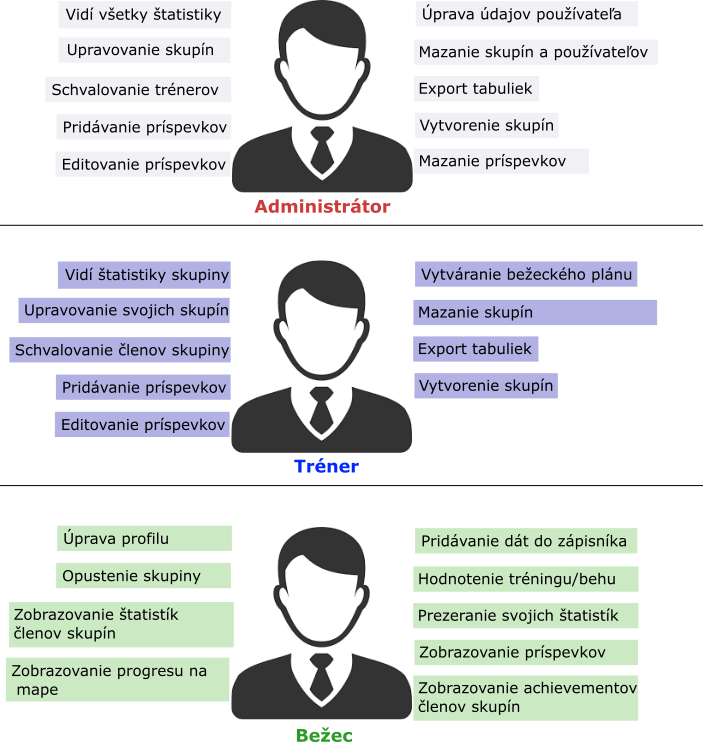
\includegraphics[width=130mm]{diagram.png}
\caption{Návrh funkcií systému \label{overflow}}
\end{figure}

\section{Triedy používateľov a ich vlastnosti}

\begin{tabular}{ll}
\hline
\multicolumn{1}{|l|}{Administrátor}    & \multicolumn{1}{l|}{\shortstack[l]{Používateľ s maximálnymi možnými právomocami na správu webovej \\ aplikácie, používateľov a skupín. Úlohou administrátora je dohliadať na \\ používateľov, pomáhať s riešením problémov, starať sa o aktuálnosť \\ informacií, schvaľovanie nových trénerov a prípadná editácia skupín a \\ používateľov.}} \\ \hline
\multicolumn{1}{|l|}{Tréner} & \multicolumn{1}{l|}{\shortstack[l]{Tréner musí byť schválený administrátorom. Jeho úlohou je spravovať \\ svoje skupiny, vytvárať bežecké plány. }}                                                  \\ \hline
\multicolumn{1}{|l|}{Bežec}        & \multicolumn{1}{l|}{\shortstack[l]{Koncový používateľ webovej aplikácie pre koho je určená. Má prístup \\ k prihláseniu, zapisovaniu svojich výsledkov do zápisníka, sledovaniu \\ svojho progresu a achievementov, prezeraniu svojich štatistík. Bežec \\ si môže prezerať profil iného bežca zo svojej skupiny. Svoj profil môže \\ kedykoľvek editovať.}                          }                                                                             \\ \hline
\end{tabular}

\section{Budúca verzia systému}
\begin{itemize}
\item Tréner bude môcť pridávať a editovať  príspevky na domovskej stránke.

\subsection{Pridávanie príspevkov na nástenku}
\begin{tabular}{ll}
\hline
\multicolumn{1}{|l|}{Popis:}    & \multicolumn{1}{l|}{\shortstack[l]{Tréner bude mať možnosť pridať príspevky na nástenku na \\ domovskej stránke aplikácie, ktoré budú viditeľné pre \\ prihlásených užívateľov.}} \\ \hline
\multicolumn{1}{|l|}{Vstupné podmienky:} & \multicolumn{1}{l|}{\shortstack[l]{-}}                                                  \\ \hline
\multicolumn{1}{|l|}{Výstupné podmienky:}& \multicolumn{1}{l|}{\shortstack[l]{-} }                                         \\ \hline
\multicolumn{1}{|l|}{Opakovanosť :} & \multicolumn{1}{l|}{\shortstack[l]{Ľubovoľná}}                                                  \\ \hline
\end{tabular}

\subsection{Editovanie príspevkov na nástenke}
\begin{tabular}{ll}
\hline
\multicolumn{1}{|l|}{Popis:}    & \multicolumn{1}{l|}{\shortstack[l]{Tréner bude mať možnosť editovať svoje príspevky na domovskej \\ stránke aplikácie.}} \\ \hline
\multicolumn{1}{|l|}{Vstupné podmienky:} & \multicolumn{1}{l|}{\shortstack[l]{-}}                                                  \\ \hline
\multicolumn{1}{|l|}{Výstupné podmienky:}& \multicolumn{1}{l|}{\shortstack[l]{-} }                                         \\ \hline
\multicolumn{1}{|l|}{Opakovanosť :} & \multicolumn{1}{l|}{\shortstack[l]{Ľubovoľná}}                                                  \\ \hline
\end{tabular}

 \item Administrátor bude môcť pridávať, editovať a mazať príspevky na domovskej stránke.

\subsection{Pridávanie príspevkov}
\begin{tabular}{ll}
\hline
\multicolumn{1}{|l|}{Popis:}    & \multicolumn{1}{l|}{\shortstack[l]{Administrátor bude mať možnosť pridávať príspevky a oznamy na hlavnú\\ stránku.}} \\ \hline
\multicolumn{1}{|l|}{Vstupné podmienky:} & \multicolumn{1}{l|}{\shortstack[l]{-}}                                                  \\ \hline
\multicolumn{1}{|l|}{Výstupné podmienky:}& \multicolumn{1}{l|}{\shortstack[l]{-} }                                         \\ \hline
\multicolumn{1}{|l|}{Opakovanosť :} & \multicolumn{1}{l|}{\shortstack[l]{Ľubovoľná}}                                                  \\ \hline
\end{tabular}

\subsection{Editovanie príspevkov}
\begin{tabular}{ll}
\hline
\multicolumn{1}{|l|}{Popis:}    & \multicolumn{1}{l|}{\shortstack[l]{Administrátor bude mať možnosť upravovať príspevky a oznamy na\\ hlavnej stránke. Ako jediný bude môcť upravovať aj príspevky trénerov.}} \\ \hline
\multicolumn{1}{|l|}{Vstupné podmienky:} & \multicolumn{1}{l|}{\shortstack[l]{-}}                                                  \\ \hline
\multicolumn{1}{|l|}{Výstupné podmienky:}& \multicolumn{1}{l|}{\shortstack[l]{-} }                                         \\ \hline
\multicolumn{1}{|l|}{Opakovanosť :} & \multicolumn{1}{l|}{\shortstack[l]{Ľubovoľná}}                                                  \\ \hline
\end{tabular}

\subsection{Mazanie príspevkov}
\begin{tabular}{ll}
\hline
\multicolumn{1}{|l|}{Popis:}    & \multicolumn{1}{l|}{\shortstack[l]{Administrátor bude mať možnosť mazať ľubovoľné príspevky a oznamy\\ na hlavnej stránke, teda aj príspevky trénerov.}} \\ \hline
\multicolumn{1}{|l|}{Vstupné podmienky:} & \multicolumn{1}{l|}{\shortstack[l]{ -}}                                                  \\ \hline
\multicolumn{1}{|l|}{Výstupné podmienky:}& \multicolumn{1}{l|}{\shortstack[l]{-} }                                         \\ \hline
\multicolumn{1}{|l|}{Opakovanosť :} & \multicolumn{1}{l|}{\shortstack[l]{Kým existuje aspoň jeden príspevok}}                                                  \\ \hline
\end{tabular}

\item Prihlasovanie pomocou Google konta.


\end{itemize}

\subsection{Zobrazovanie Achievementov}
\begin{tabular}{ll}
\hline
\multicolumn{1}{|l|}{Popis:}    & \multicolumn{1}{l|}{\shortstack[l]{Bežec dostáva po splnení určeného cieľa (napr. zabehnúť spolu 50km)\\ achievement.  Čím viacej sa bežec snaží napredovať, tým výnimočnejší\\ achievement dostane, čo by ho malo motivovať k ďaľším výkonom.}} \\ \hline
\multicolumn{1}{|l|}{Vstupné podmienky:} & \multicolumn{1}{l|}{\shortstack[l]{ - }}                                                  \\ \hline
\multicolumn{1}{|l|}{Výstupné podmienky:}& \multicolumn{1}{l|}{\shortstack[l]{-} }                                         \\ \hline
\multicolumn{1}{|l|}{Opakovanosť :} & \multicolumn{1}{l|}{\shortstack[l]{Preddefinovaná}}                                                  \\ \hline
\end{tabular}

\subsection{Zobrazenie štatistík skupiny}
\begin{tabular}{ll}
\hline
\multicolumn{1}{|l|}{Popis:}    & \multicolumn{1}{l|}{\shortstack[l]{Tréner bude mať možnosť zobrazovať štatistiky svojich skupín.}} \\ \hline
\multicolumn{1}{|l|}{Vstupné podmienky:} & \multicolumn{1}{l|}{\shortstack[l]{-}}                                                  \\ \hline
\multicolumn{1}{|l|}{Výstupné podmienky:}& \multicolumn{1}{l|}{\shortstack[l]{-} }                                         \\ \hline
\multicolumn{1}{|l|}{Opakovanosť :} & \multicolumn{1}{l|}{\shortstack[l]{Ľubovoľná}}                                                  \\ \hline
\end{tabular}

\subsection{Export tabuliek}
\begin{tabular}{ll}
\hline
\multicolumn{1}{|l|}{Popis:}    & \multicolumn{1}{l|}{\shortstack[l]{Tréner bude mať možnosť vyexportovať tabuľky so štatistikami \\ jeho skupiny.}} \\ \hline
\multicolumn{1}{|l|}{Vstupné podmienky:} & \multicolumn{1}{l|}{\shortstack[l]{-}}                                                  \\ \hline
\multicolumn{1}{|l|}{Výstupné podmienky:}& \multicolumn{1}{l|}{\shortstack[l]{-} }                                         \\ \hline
\multicolumn{1}{|l|}{Opakovanosť :} & \multicolumn{1}{l|}{\shortstack[l]{Ľubovoľná}}                                                  \\ \hline
\end{tabular}


\subsection{Zobrazovanie príspevkov na domovskej stránke}
\begin{tabular}{ll}
\hline
\multicolumn{1}{|l|}{Popis:}    & \multicolumn{1}{l|}{\shortstack[l]{Používateľ bude mať možnosť vidieť všetky aktuálne príspevky a \\ oznamy od trénerov. }} \\ \hline
\multicolumn{1}{|l|}{Vstupné podmienky:} & \multicolumn{1}{l|}{\shortstack[l]{ - }}                                                  \\ \hline
\multicolumn{1}{|l|}{Výstupné podmienky:}& \multicolumn{1}{l|}{\shortstack[l]{-} }                                         \\ \hline
\multicolumn{1}{|l|}{Opakovanosť :} & \multicolumn{1}{l|}{\shortstack[l]{Ľubovoľná}}                                                  \\ \hline
\end{tabular}


\chapter{Špecifikácia požiadaviek}

\section{Možnosti bežca po prihlásení}


\subsection{Zobrazovanie štatistík}
\begin{tabular}{ll}
\hline
\multicolumn{1}{|l|}{Popis:}    & \multicolumn{1}{l|}{\shortstack[l]{Používateľ bude mať možnosť vidieť tabuľku so svojími výkonmi.\\Bude si môcť vybrať aj tímové štatistiky, kde nebude vidieť \\ jednotlivých členov, ale výkon ako celku a koľkým \\i percentami prispel k tomuto výkonu. }} \\ \hline
\multicolumn{1}{|l|}{Vstupné podmienky:} & \multicolumn{1}{l|}{\shortstack[l]{- }}                                                  \\ \hline
\multicolumn{1}{|l|}{Výstupné podmienky:}& \multicolumn{1}{l|}{\shortstack[l]{-} }                                         \\ \hline
\multicolumn{1}{|l|}{Opakovanosť :} & \multicolumn{1}{l|}{\shortstack[l]{Ľubovoľná}}                                                  \\ \hline
\end{tabular}

\subsection{Výber plánu}
\begin{tabular}{ll}
\hline
\multicolumn{1}{|l|}{Popis:}    & \multicolumn{1}{l|}{\shortstack[l]{Bežec dostáva možnosť prihlásiť sa do bežeckého plánu zadaného\\ trénerom. Bežec môže byť pridelený k plánu už priamo ténerom. }} \\ \hline
\multicolumn{1}{|l|}{Vstupné podmienky:} & \multicolumn{1}{l|}{\shortstack[l]{ - }}                                                  \\ \hline
\multicolumn{1}{|l|}{Výstupné podmienky:}& \multicolumn{1}{l|}{\shortstack[l]{-} }                                         \\ \hline
\multicolumn{1}{|l|}{Opakovanosť :} & \multicolumn{1}{l|}{\shortstack[l]{Preddefinovaná}}                                                  \\ \hline
\end{tabular}

\subsection{Vkladanie údajov do zápisníka}
\begin{tabular}{ll}
\hline
\multicolumn{1}{|l|}{Popis:}    & \multicolumn{1}{l|}{\shortstack[l]{Používateľovi sa zobrazí formulár, do ktorého zadá dátum, koľko \\ kilometrov zabehol, môže pridať komentár a  ohodnotiť tréning \\ pomocou smajlíkov. Po zadaní údajov sa kilometre pripočítajú \\ k tímovej štatistike a bežec bude môcť na mape sledovať o kolko \\ sa jeho tím posunul v napĺňaní svojho bežeckého\\ plánu k dosiahnutiu cieľa. }} \\ \hline
\multicolumn{1}{|l|}{Vstupné podmienky:} & \multicolumn{1}{l|}{\shortstack[l]{- }}                                                  \\ \hline
\multicolumn{1}{|l|}{Výstupné podmienky:}& \multicolumn{1}{l|}{\shortstack[l]{-} }                                         \\ \hline
\multicolumn{1}{|l|}{Opakovanosť :} & \multicolumn{1}{l|}{\shortstack[l]{Ľubovoľná}}                                                  \\ \hline
\end{tabular}



\subsection{Zobrazovanie profilu bežca}
\begin{tabular}{ll}
\hline
\multicolumn{1}{|l|}{Popis:}    & \multicolumn{1}{l|}{\shortstack[l]{Bežec má už po vyplnení registrácie svoj vlastný profil, \\ ktorý obsahuje základné informácie o bežcovi ako napr. meno,\\ vek, kontaktné údaje a fotku.\\ Bežec si môže prezerať aj profil iných členov skupiny a svojho trénera.}} \\ \hline
\multicolumn{1}{|l|}{Vstupné podmienky:} & \multicolumn{1}{l|}{\shortstack[l]{- }}                                                  \\ \hline
\multicolumn{1}{|l|}{Výstupné podmienky:}& \multicolumn{1}{l|}{\shortstack[l]{-} }                                         \\ \hline
\multicolumn{1}{|l|}{Opakovanosť :} & \multicolumn{1}{l|}{\shortstack[l]{Ľubovoľná}}                                                  \\ \hline
\end{tabular}

\subsection{Upravenie profilu}
\begin{tabular}{ll}
\hline
\multicolumn{1}{|l|}{Popis:}    & \multicolumn{1}{l|}{\shortstack[l]{Každý bežec môže upravovať svoj profil, teda vybrať si jedného \\ zo skupiny avatarov, zmeniť názov školy, \\ upraviť dátum narodenia, prípadne pridať kontaktné údaje. }} \\ \hline
\multicolumn{1}{|l|}{Vstupné podmienky:} & \multicolumn{1}{l|}{\shortstack[l]{ - }}                                                  \\ \hline
\multicolumn{1}{|l|}{Výstupné podmienky:}& \multicolumn{1}{l|}{\shortstack[l]{-} }                                         \\ \hline
\multicolumn{1}{|l|}{Opakovanosť :} & \multicolumn{1}{l|}{\shortstack[l]{Ľubovoľná}}                                                  \\ \hline
\end{tabular}

\subsection{Opustenie skupiny}
\begin{tabular}{ll}
\hline
\multicolumn{1}{|l|}{Popis:}    & \multicolumn{1}{l|}{\shortstack[l]{Každý bežec môže opustiť svoju skupinu. Po opustení skupiny \\ bude musieť požiadať trénera aby mu pridelil novú skupinu.}} \\ \hline
\multicolumn{1}{|l|}{Vstupné podmienky:} & \multicolumn{1}{l|}{\shortstack[l]{- }}                                                  \\ \hline
\multicolumn{1}{|l|}{Výstupné podmienky:}& \multicolumn{1}{l|}{\shortstack[l]{-} }                                         \\ \hline
\multicolumn{1}{|l|}{Opakovanosť :} & \multicolumn{1}{l|}{\shortstack[l]{Jednorázová}}                                                  \\ \hline
\end{tabular}

\section{Možnosti trénera po prihlásení}

\subsection{Schvaľovanie členov skupiny}
\begin{tabular}{ll}
\hline
\multicolumn{1}{|l|}{Popis:}    & \multicolumn{1}{l|}{\shortstack[l]{Tréner bude mať možnosť schváliť alebo odmietnuť požiadavku \\ o vstup užívateľa do jeho skupiny. Požiadavka sa objaví po tom \\ ako si užívateľ vyberie svojho trénera. Každú požiadavku je \\ možné prijať/odmietnuť raz pre jeden užívateľov výber trénera.}} \\ \hline
\multicolumn{1}{|l|}{Vstupné podmienky:} & \multicolumn{1}{l|}{\shortstack[l]{Užívateľ pošle požiadavku pomocou výberu trénera}}                                                  \\ \hline
\multicolumn{1}{|l|}{Výstupné podmienky:}& \multicolumn{1}{l|}{\shortstack[l]{-} }                                         \\ \hline
\multicolumn{1}{|l|}{Opakovanosť :} & \multicolumn{1}{l|}{\shortstack[l]{V závislosti od požiadaviek.}}                                                  \\ \hline
\end{tabular}

\subsection{Vytváranie bežeckého plánu}
\begin{tabular}{ll}
\hline
\multicolumn{1}{|l|}{Popis:}    & \multicolumn{1}{l|}{\shortstack[l]{Tréner bude mať možnosť vytvoriť bežecký plán pre svoju skupinu \\ zvolením trasi na mape. Cieľom bežca je odbehnúť počet \\ kilometrov určený touto trasou. Tréner vyberie bežcov pre\\ aktuálny plán, alebo sa bežec prihlási sám.}} \\ \hline
\multicolumn{1}{|l|}{Vstupné podmienky:} & \multicolumn{1}{l|}{\shortstack[l]{-}}                                                  \\ \hline
\multicolumn{1}{|l|}{Výstupné podmienky:}& \multicolumn{1}{l|}{\shortstack[l]{-} }                                         \\ \hline
\multicolumn{1}{|l|}{Opakovanosť :} & \multicolumn{1}{l|}{\shortstack[l]{Ľubovoľná}}                                                  \\ \hline
\end{tabular}

\subsection{Mazanie skupín}
\begin{tabular}{ll}
\hline
\multicolumn{1}{|l|}{Popis:}    & \multicolumn{1}{l|}{\shortstack[l]{Tréner bude mať možnosť zmazať svoju skupinu.}} \\ \hline
\multicolumn{1}{|l|}{Vstupné podmienky:} & \multicolumn{1}{l|}{\shortstack[l]{-}}                                                  \\ \hline
\multicolumn{1}{|l|}{Výstupné podmienky:}& \multicolumn{1}{l|}{\shortstack[l]{-} }                                         \\ \hline
\multicolumn{1}{|l|}{Opakovanosť :} & \multicolumn{1}{l|}{\shortstack[l]{Kým existuje aspoň jedna skupina vytvorená trénerom.}}                                                  \\ \hline
\end{tabular}

\subsection{Upravovanie skupín}
\begin{tabular}{ll}
\hline
\multicolumn{1}{|l|}{Popis:}    & \multicolumn{1}{l|}{\shortstack[l]{Tréner bude mať možnosť upravovať svoje skupiny.}} \\ \hline
\multicolumn{1}{|l|}{Vstupné podmienky:} & \multicolumn{1}{l|}{\shortstack[l]{-}}                                                  \\ \hline
\multicolumn{1}{|l|}{Výstupné podmienky:}& \multicolumn{1}{l|}{\shortstack[l]{-} }                                         \\ \hline
\multicolumn{1}{|l|}{Opakovanosť :} & \multicolumn{1}{l|}{\shortstack[l]{Kým existuje aspoň jedna skupina vytvorená trénerom.}}                                                  \\ \hline
\end{tabular}



\subsection{Vytvorenie skupín}
\begin{tabular}{ll}
\hline
\multicolumn{1}{|l|}{Popis:}    & \multicolumn{1}{l|}{\shortstack[l]{Tréner bude mať možnosť vytvoriť skupinu.}} \\ \hline
\multicolumn{1}{|l|}{Vstupné podmienky:} & \multicolumn{1}{l|}{\shortstack[l]{-}}                                                  \\ \hline
\multicolumn{1}{|l|}{Výstupné podmienky:}& \multicolumn{1}{l|}{\shortstack[l]{-} }                                         \\ \hline
\multicolumn{1}{|l|}{Opakovanosť :} & \multicolumn{1}{l|}{\shortstack[l]{Ľubovoľná}}                                                  \\ \hline
\end{tabular}

\section{Možnosti administrátora po prihlásení}



%\subsection{Vytvorenie skupiny}
%\begin{tabular}{ll}
%\hline
%\multicolumn{1}{|l|}{Popis:}    & \multicolumn{1}{l|}{\shortstack[l]{Administrátor bude mať možnosť podobne ako tréner vytvoriť skupinu,\\ ktorej pridelí trénera.}} \\ \hline
%\multicolumn{1}{|l|}{Vstupné podmienky:} & \multicolumn{1}{l|}{\shortstack[l]{-}}                                                  \\ \hline
%\multicolumn{1}{|l|}{Výstupné podmienky:}& \multicolumn{1}{l|}{\shortstack[l]{-} }                                         \\ \hline
%\multicolumn{1}{|l|}{Opakovanosť :} & \multicolumn{1}{l|}{\shortstack[l]{Ľubovoľná}}                                                  \\ \hline
%\end{tabular}

%\subsection{Editovanie skupiny}
%\begin{tabular}{ll}
%\hline
%\multicolumn{1}{|l|}{Popis:}    & \multicolumn{1}{l|}{\shortstack[l]{Administrátor bude mať možnosť upravovať skupinu.}} \\ \hline
%\multicolumn{1}{|l|}{Vstupné podmienky:} & \multicolumn{1}{l|}{\shortstack[l]{-}}                                                  \\ \hline
%\multicolumn{1}{|l|}{Výstupné podmienky:}& \multicolumn{1}{l|}{\shortstack[l]{-} }                                         \\ \hline
%\multicolumn{1}{|l|}{Opakovanosť :} & \multicolumn{1}{l|}{\shortstack[l]{Ľubovoľná}}                                                  \\ \hline
%\end{tabular}
%
%\subsection{Mazanie skupiny}
%\begin{tabular}{ll}
%\hline
%\multicolumn{1}{|l|}{Popis:}    & \multicolumn{1}{l|}{\shortstack[l]{Administrátor bude mať možnosť zmazať skupinu.}} \\ \hline
%\multicolumn{1}{|l|}{Vstupné podmienky:} & \multicolumn{1}{l|}{\shortstack[l]{-}}                                                  \\ \hline
%\multicolumn{1}{|l|}{Výstupné podmienky:}& \multicolumn{1}{l|}{\shortstack[l]{-} }                                         \\ \hline
%\multicolumn{1}{|l|}{Opakovanosť :} & \multicolumn{1}{l|}{\shortstack[l]{Kým existuje aspoň jedna skupina}}                                                  \\ \hline
%\end{tabular}
%
%\subsection{Editovanie používateľa}
%\begin{tabular}{ll}
%\hline
%\multicolumn{1}{|l|}{Popis:}    & \multicolumn{1}{l|}{\shortstack[l]{Administrátor bude mať možnosť upravovať údaje používateľa. Nebude môcť \\meniť email a heslo, nakoľko bude použité google api.}} \\ \hline
%\multicolumn{1}{|l|}{Vstupné podmienky:} & \multicolumn{1}{l|}{\shortstack[l]{-}}                                                  \\ \hline
%\multicolumn{1}{|l|}{Výstupné podmienky:}& \multicolumn{1}{l|}{\shortstack[l]{-} }                                         \\ \hline
%\multicolumn{1}{|l|}{Opakovanosť :} & \multicolumn{1}{l|}{\shortstack[l]{Ľubovoľná}}                                                  \\ \hline
%\end{tabular}

\subsection{Zmazanie používateľa}
\begin{tabular}{ll}
\hline
\multicolumn{1}{|l|}{Popis:}    & \multicolumn{1}{l|}{\shortstack[l]{Administrátor bude mať možnosť vymazať používateľa z databázy\\ používateľov.}} \\ \hline
\multicolumn{1}{|l|}{Vstupné podmienky:} & \multicolumn{1}{l|}{\shortstack[l]{-}}                                                  \\ \hline
\multicolumn{1}{|l|}{Výstupné podmienky:}& \multicolumn{1}{l|}{\shortstack[l]{-} }                                         \\ \hline
\multicolumn{1}{|l|}{Opakovanosť :} & \multicolumn{1}{l|}{\shortstack[l]{Kým existuje aspoň jeden používateľ}}                                                  \\ \hline
\end{tabular}

\subsection{Aktivovanie používateľa}
\begin{tabular}{ll}
\hline
\multicolumn{1}{|l|}{Popis:}    & \multicolumn{1}{l|}{\shortstack[l]{Administrátor bude mať možnosť aktivovať používateľa.}} \\ \hline
\multicolumn{1}{|l|}{Vstupné podmienky:} & \multicolumn{1}{l|}{\shortstack[l]{-}}                                                  \\ \hline
\multicolumn{1}{|l|}{Výstupné podmienky:}& \multicolumn{1}{l|}{\shortstack[l]{-} }                                         \\ \hline
\multicolumn{1}{|l|}{Opakovanosť :} & \multicolumn{1}{l|}{\shortstack[l]{Kým existuje aspoň jeden neaktívny používateľ}}                                                  \\ \hline
\end{tabular}

\subsection{Schvaľovanie trénerov}
\begin{tabular}{ll}
\hline
\multicolumn{1}{|l|}{Popis:}    & \multicolumn{1}{l|}{\shortstack[l]{Aby sa bežný používateľ mohol stať trénerom, musí jeho žiadosť\\ schváliť (alebo zamietnuť) administrátor.}} \\ \hline
\multicolumn{1}{|l|}{Vstupné podmienky:} & \multicolumn{1}{l|}{\shortstack[l]{-}}                                                  \\ \hline
\multicolumn{1}{|l|}{Výstupné podmienky:}& \multicolumn{1}{l|}{\shortstack[l]{-} }                                         \\ \hline
\multicolumn{1}{|l|}{Opakovanosť :} & \multicolumn{1}{l|}{\shortstack[l]{V závislosti od požiadaviek}}                                                  \\ \hline
\end{tabular}

\subsection{Rušenie trénerov}
\begin{tabular}{ll}
\hline
\multicolumn{1}{|l|}{Popis:}    & \multicolumn{1}{l|}{\shortstack[l]{Administrátor bude mať možnosť zbaviť používateľa trénerských funkcionalít.}} \\ \hline
\multicolumn{1}{|l|}{Vstupné podmienky:} & \multicolumn{1}{l|}{\shortstack[l]{-}}                                                  \\ \hline
\multicolumn{1}{|l|}{Výstupné podmienky:}& \multicolumn{1}{l|}{\shortstack[l]{-} }                                         \\ \hline
\multicolumn{1}{|l|}{Opakovanosť :} & \multicolumn{1}{l|}{\shortstack[l]{Kým existuje aspoň jeden aktívny tréner.}}                                                  \\ \hline
\end{tabular}

%\subsection{Zobrazovanie štatistík}
%\begin{tabular}{ll}
%\hline
%\multicolumn{1}{|l|}{Popis:}    & \multicolumn{1}{l|}{\shortstack[l]{Administrátor, ako jediný, má možnosť vidieť štatistiky a výsledky\\ všetkých bežcov.}} \\ \hline
%\multicolumn{1}{|l|}{Vstupné podmienky:} & \multicolumn{1}{l|}{\shortstack[l]{-}}                                                  \\ \hline
%\multicolumn{1}{|l|}{Výstupné podmienky:}& \multicolumn{1}{l|}{\shortstack[l]{-} }                                         \\ \hline
%\multicolumn{1}{|l|}{Opakovanosť :} & \multicolumn{1}{l|}{\shortstack[l]{Ľubovoľná}}                                                  \\ \hline
%\end{tabular}
%
%\subsection{Zobrazovanie profilov}
%\begin{tabular}{ll}
%\hline
%\multicolumn{1}{|l|}{Popis:}    & \multicolumn{1}{l|}{\shortstack[l]{Administrátor, ako jediný, má možnosť vidieť profil každého bežca.}} \\ \hline
%\multicolumn{1}{|l|}{Vstupné podmienky:} & \multicolumn{1}{l|}{\shortstack[l]{-}}                                                  \\ \hline
%\multicolumn{1}{|l|}{Výstupné podmienky:}& \multicolumn{1}{l|}{\shortstack[l]{-} }                                         \\ \hline
%\multicolumn{1}{|l|}{Opakovanosť :} & \multicolumn{1}{l|}{\shortstack[l]{Ľubovoľná}}                                                  \\ \hline
%\end{tabular}
%
%\subsection{Export tabuliek}
%\begin{tabular}{ll}
%\hline
%\multicolumn{1}{|l|}{Popis:}    & \multicolumn{1}{l|}{\shortstack[l]{Administrátor bude mať možnosť vyexportovať tabuľky so štatistikami \\ ktorejkoľvek skupiny.}} \\ \hline
%\multicolumn{1}{|l|}{Vstupné podmienky:} & \multicolumn{1}{l|}{\shortstack[l]{-}}                                                  \\ \hline
%\multicolumn{1}{|l|}{Výstupné podmienky:}& \multicolumn{1}{l|}{\shortstack[l]{-} }                                         \\ \hline
%\multicolumn{1}{|l|}{Opakovanosť :} & \multicolumn{1}{l|}{\shortstack[l]{Ľubovoľná}}                                                  \\ \hline
%\end{tabular}

%TODO: MOZNO DAT PREC EXPORT TAB, ZOBRAZ. PROF.,  ZOBRAZ STATS, EDITOVANIE POUZ.


\chapter{Ďaľšie požiadavky}

\section{Výkonostné požiadavky}

\begin{itemize}  
\item Webová aplikácia bude spracovávať údaje členov jedného bežeckého klubu. 
\item Predpokladaný počet je maximálne 1000 členov
\item Počet dotazov na Google-maps api nepresiahne 2500/deň 
\end{itemize}

\section{Dostupnosť}
\begin{itemize}  
\item Dostupnosť servera aspoň 97\%
\end{itemize}

\section{Bezpečnostné požiadavky}
\begin{itemize}  
\item Zobrazenie profilov a obsahu až po registrácii alebo prihlásení
\item Na prihlasovanie používanie Google api
\item Schvaľovanie a kontrola administrátorom 
\item Obmedzené prístupové práva pre bežcov a trénerov
\end{itemize}

\chapter{Analýza technológií}

\section{HTML}
\begin{itemize}
\item HTML (Hypertext Markup Language) bude použité na základnú štruktúru webovej aplikácie a rozmiestnenie objektov.
\item využitá bude verzia HTML 5.0
\item HTML bude kombinované s viacerými jazykmi, ako napríklad PHP, CSS...
\end{itemize}

\section{CSS}
\begin{itemize}
\item CSS (Cascading Style Sheets) bude použité na vytvorenie, úpravu dizajnu a štylizovanie webovej aplikácie.
\item využitá bude verzia CSS 3.0
\item CSS bude využité aj na vytvorenie responzivity webovej aplikácie
\end{itemize}

\section{Bootstrap}
\begin{itemize}
\item Bootstrap je jednoduchá voľne stiahnuteľná sada nástrojov na tvorbu webových aplikácií
\item obsahuje návrhárske šablóny založené na HTML a CSS
\item pre využívanie je potrebná dobrá znalosť HTML a CSS
\item využíva LESS deklarácie, čo umožňuje používanie napr. premenných a funkcií priamo v CSS kóde
\item dôvod použitia: efektívnejšia práca pri navrhovaní a vytváraní responzívnej aplikácie
\end{itemize}

\section{LESS}
\begin{itemize}
\item LESS je "dynamic style sheet"  jazyk, ktorý je možné skompilovať do CSS
\item umožňuje definovať a používať premenné a funkcie
\item dôvod použitia: efektívnejšia práca pri úpravách CSS, eliminácia duplicity (napr. zmena farieb...)
\end{itemize}

\section{PHP}
\begin{itemize}
\item PHP je skriptovací jazyk, ktorý sa používa najmä na programovanie klient-server aplikácií
\item dôvod použitia: PHP dokáže spolupracovať s relačnými databázami, ako napr. MySQL alebo SQLite, ktoré budú súčasťou nášho projektu
\item predpokladané použitie verzie PHP 5.5 / 7
\end{itemize}

\section{JavaScript}
\begin{itemize}
\item JS je multiplatformový, objektovo orientovaný skriptovací jazyk na strane klienta
\item dôvod použitia: využitie na interakciu s používateľom, prácu s dátami z GoogleMaps API 
\end{itemize}

\section{Laravel}
\begin{itemize}
\item open source framework pre PHP
\item Laravel zahŕňa ako základné funkcie:
	
	\begin{itemize}
	\item autentifikáciu - kontrolu prístupu
	\item routovanie - spravovanie, smerovanie a spracovanie dotazov na jednom mieste
	\item databázu - všetky nástroje potrebné na komunikáciu s databázou
	\item mail - posielanie emailov s prílohami a vloženými súbormi
	\item sessions
	\item caching 
	\end{itemize}

\item dôvod použitia: zjednodušenie práce pri programovaní funkcií, bezpečnejšie a efektívnejšie algoritmy na autentifikáciu a komunikáciu s databázou
\end{itemize}

\section{SQL}
\begin{itemize}
\item štruktúrovaný dopytovací jazyk určený na manipuláciu (výber, vkladanie, úpravu a mazanie) a definúciu údajov v relačných databázových systémoch
\item dôvod použitia: jedna z hlavných súčastí projektu budú relačné databázy a práca s nimi
\end{itemize}

\section{SQLite}
\begin{itemize}
\item je relačná databáza pracujúca bez servera, čiže používa iba klientsku časť
\item nie je potrebná jej inštalácia ani žiadne konfiguračné súbory
\item jednoduchý import a export tabuliek
\item dôvod použitia: využitie na uloženie dát potrebných pre fungovanie webovej aplikácie
\end{itemize}

\section{WAMP / LAMP}
\begin{itemize}
\item apache, MySQL a PHP aplikačná serverová platforma
\item dôvod použitia: využitie počas testovania webovej aplikácie bez prístupu k serveru, na ktorom bude výsledná aplikácia bežať
\end{itemize}

\chapter{Diagramy}
\section{Use-case diagram}
\begin{figure}[h]
\centering
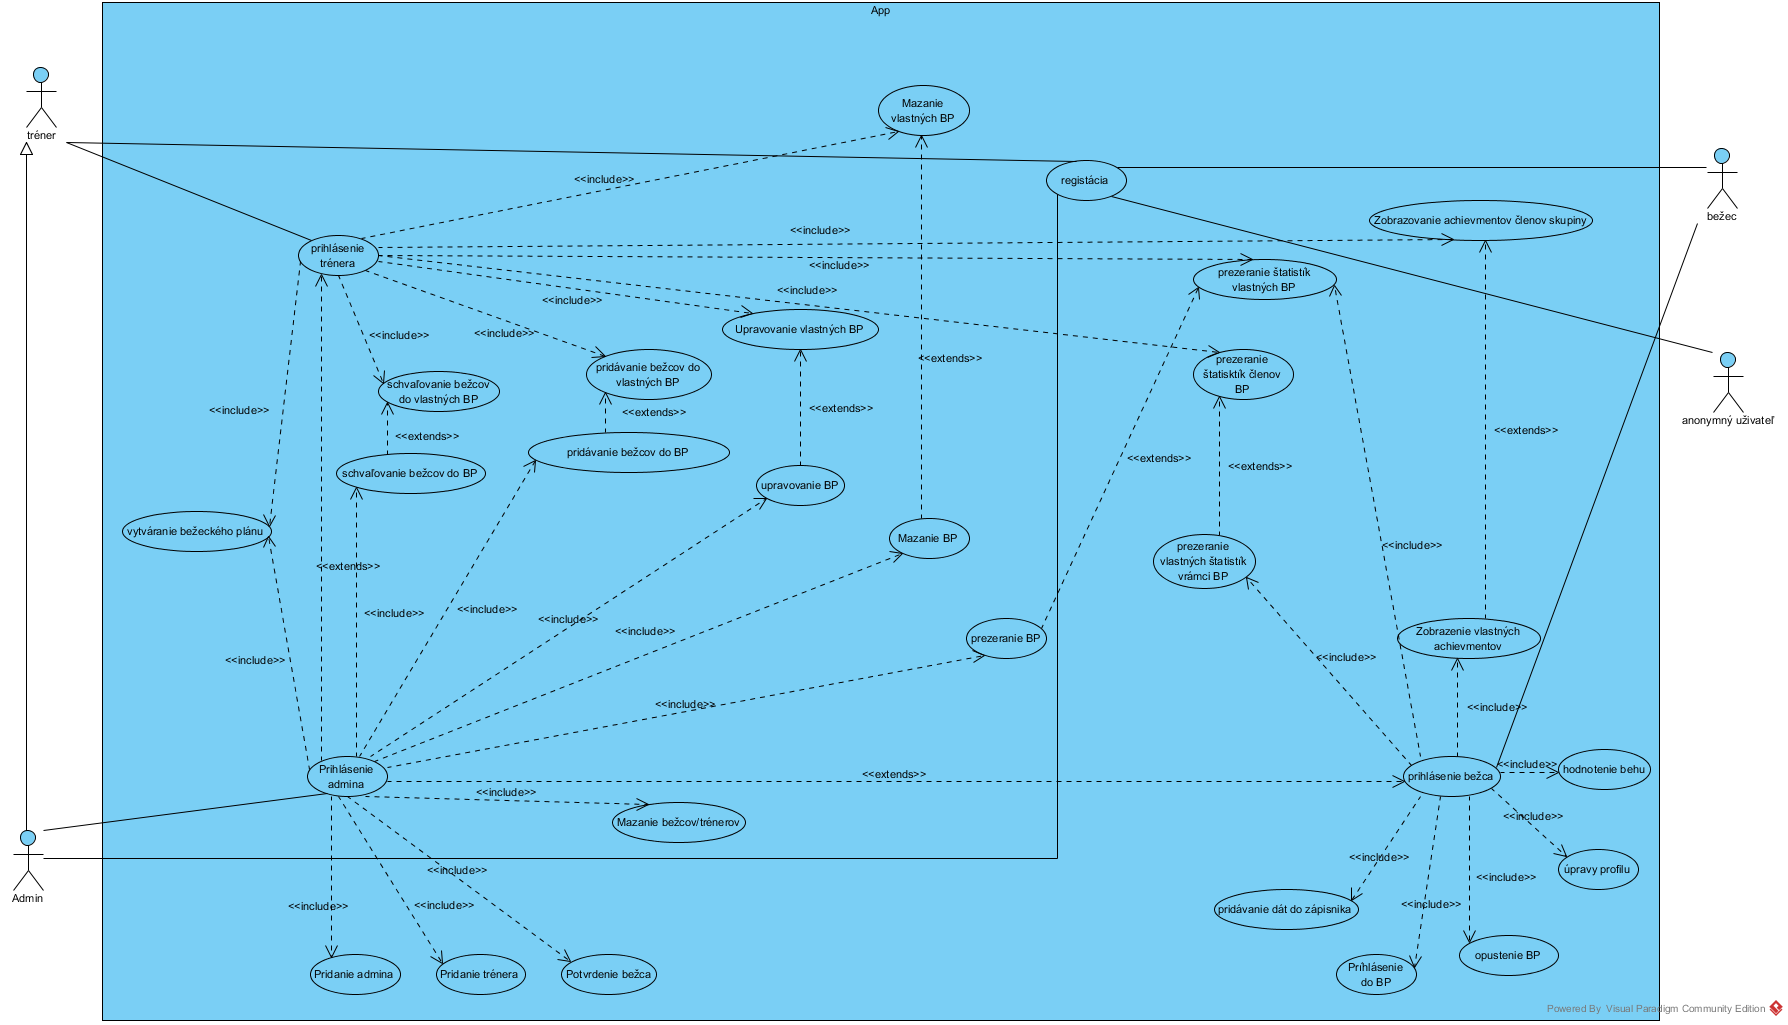
\includegraphics[width=\textwidth]{UseCaseDiagram1.png}
\caption{Use-case diagram}
\end{figure}

Používateľ aplikácie je buď tréner, admin, bežec alebo anonymný používateľ. Anonymný používateľ má možnosť sa len registrovať kedže aplikácia má funkcie prístupné len po prihlásení. Bežec si po prihlásení môže prezerať svoje štatistiky a aj štatisktiky svojej skupiny, takisto si môže prezerať  achievmenty seba aj skupiny, môže hodnotiť beh, upravovať profil a prihlasovať a opúštať skupiny. Tréner aj admin môžu vytvárať, upravovať a mazať skupiny, schvalovať a pridávať bežcov do skupín a prezerať si štatisky skupín s tým, že tréner má tieto funkcie povolené len pre vlastné skupiny a bežecké plány. Admin môže ešte navyše aj pridávať potvrdzovať a mazať užívateľov.

Tento diagram zachytáva aj funkcie, ktoré bude implementované až v ďaľších verziách.

\newpage
\section{Entitno-relačný diagram}
\begin{figure}[H]
\centering
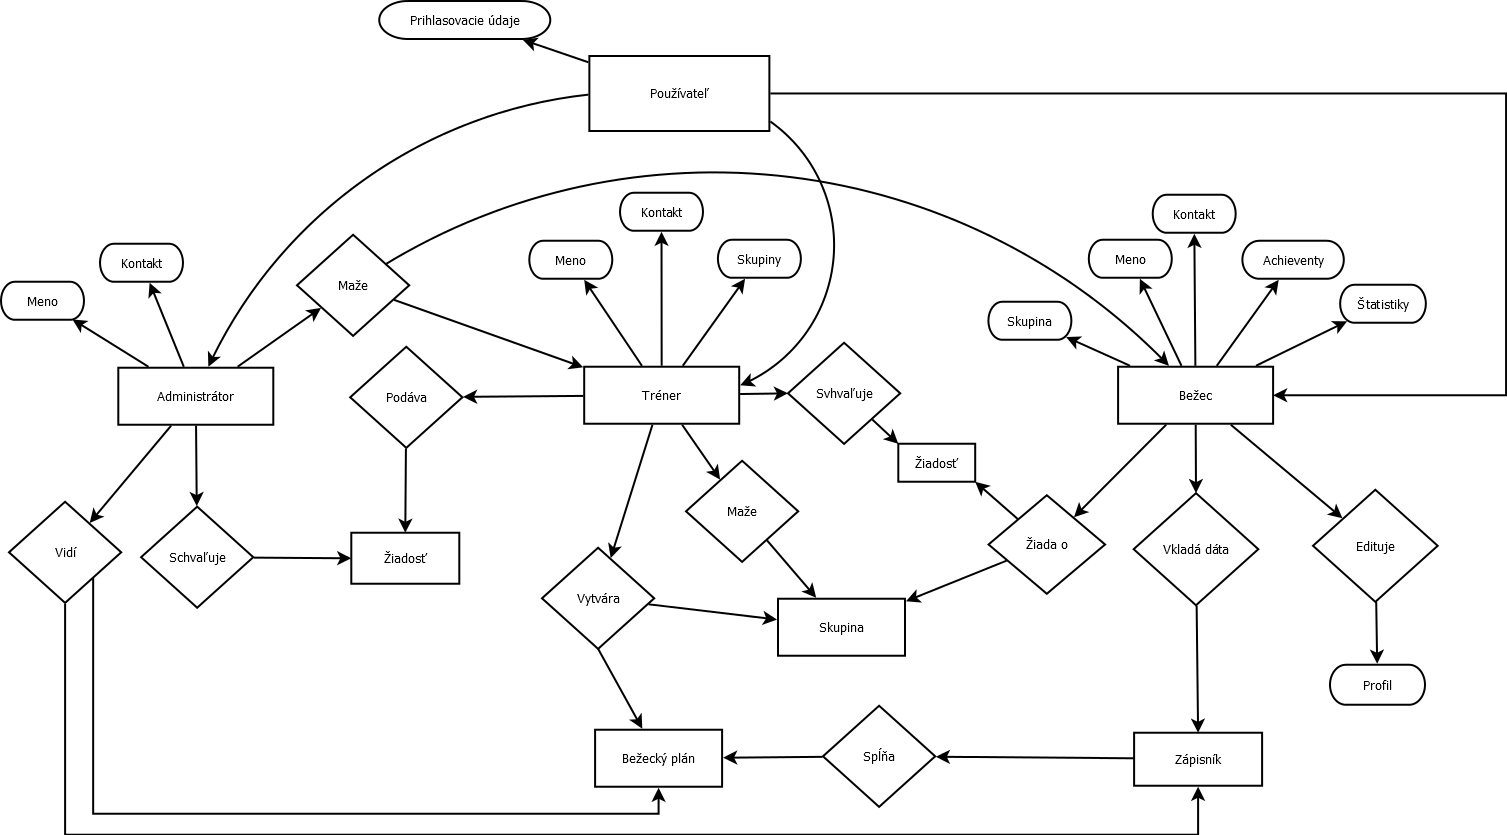
\includegraphics[width=\textwidth]{ERdiagram.png}
\caption{ERD}
\end{figure}

Entitno-relačný diagram ( obr 2.2 ) zobrazuje entity vystupujúce v systéme a relácie ( vzťahy ) medzi nimi. Diagram slúži pre lepšiu orientáciu počas návrhu dátového diagramu ( databázy ) a aj počas navrhovania diagramov popisujúcich samotnú funkcionalitu systému. ER diagram znázorňuje delenie používateľov do troch skupín na Administrátora, Trénera a Bežca a popisuje jednotlivé kľúčové funkcie a atribúty ktoré bude aplikácia obsahovať.

 \newpage
\section{Stavové diagramy}
\begin{figure}[!htb]
\centering
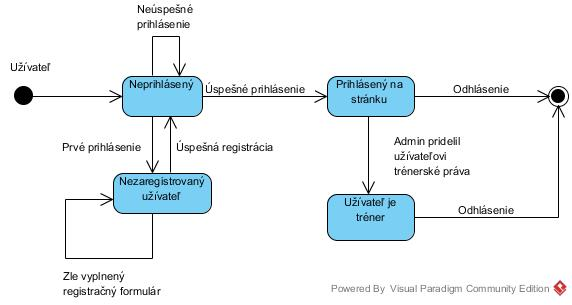
\includegraphics[width=\textwidth]{State diagram - user.jpg}
\caption{User state diagram}
\end{figure}

Stavový diagram užívateľa ( obr. 2.3 ) zobrazuje pasívne stavy užívateľa v systéme a udalosti/akcie, na základe ktorých sa dostáva do iného stavu.

\begin{figure}[!htb]
\centering
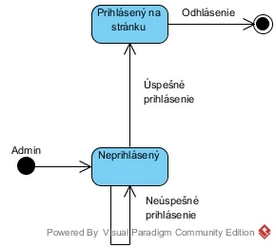
\includegraphics{State diagram - admin.jpg}
\caption{Admin state diagram}
\end{figure}

Stavový diagram admina ( obr. 2.4 ) zobrazuje pasívne stavy admina v systéme a udalosti/akcie, na základe ktorých sa dostáva do iného stavu.


\newpage
\section{Sekvenčný diagram}
\begin{figure}[H]
\centering
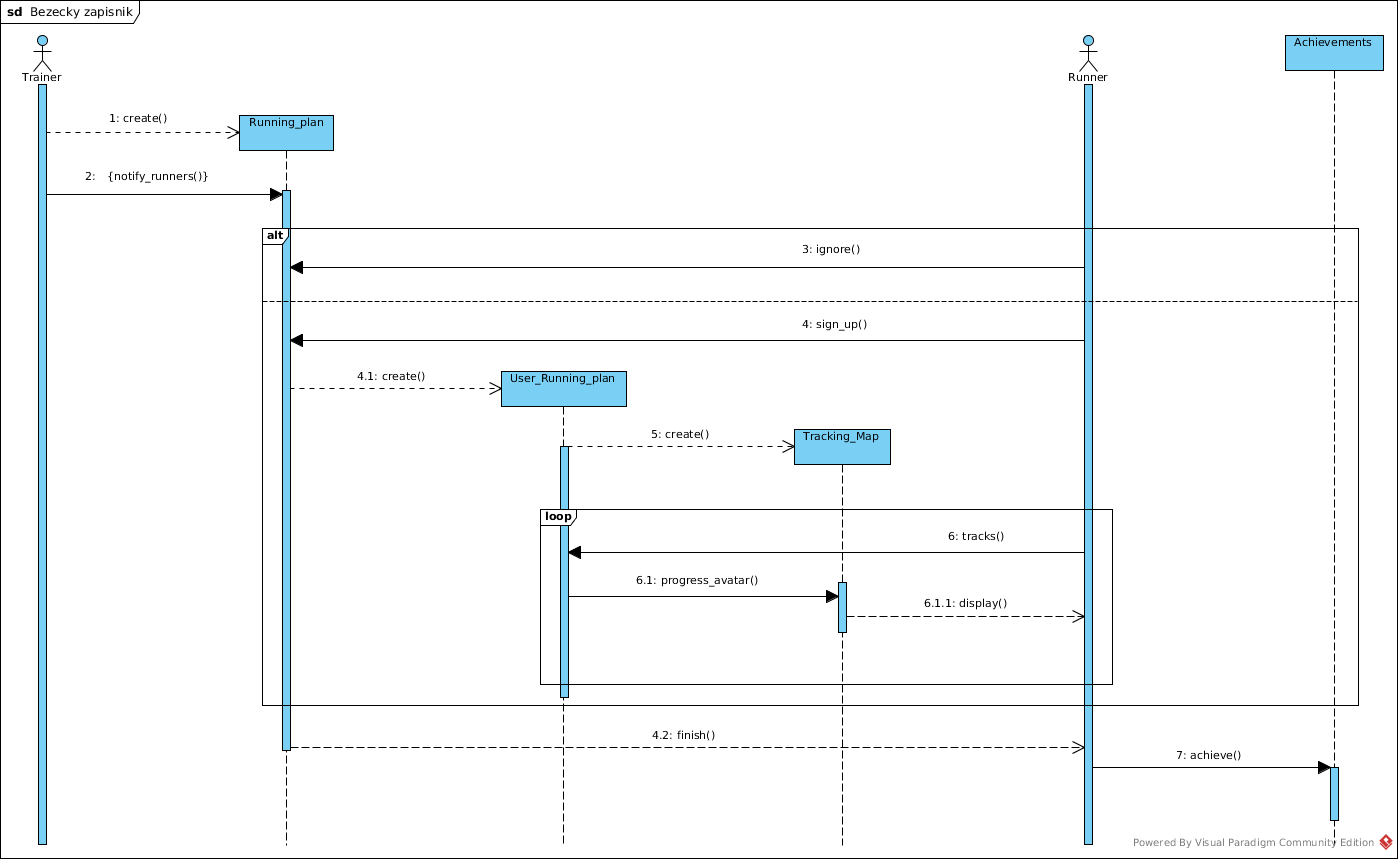
\includegraphics[width=\textwidth]{Bezecky zapisnik.png}
\caption{Sekvenčný diagram}
\end{figure}

Sekvenčný diagram ( obr. 2.5 ) graficky zachytáva sled nadväzných udalostí zaznačovania pokroku v plnení bežeckého plánu, vytvoreného trénerom a postupnými iteráciami napĺňajúceho sa bežcom.

\newpage
\section{Triedny diagram}
\begin{figure}[H]
\centering
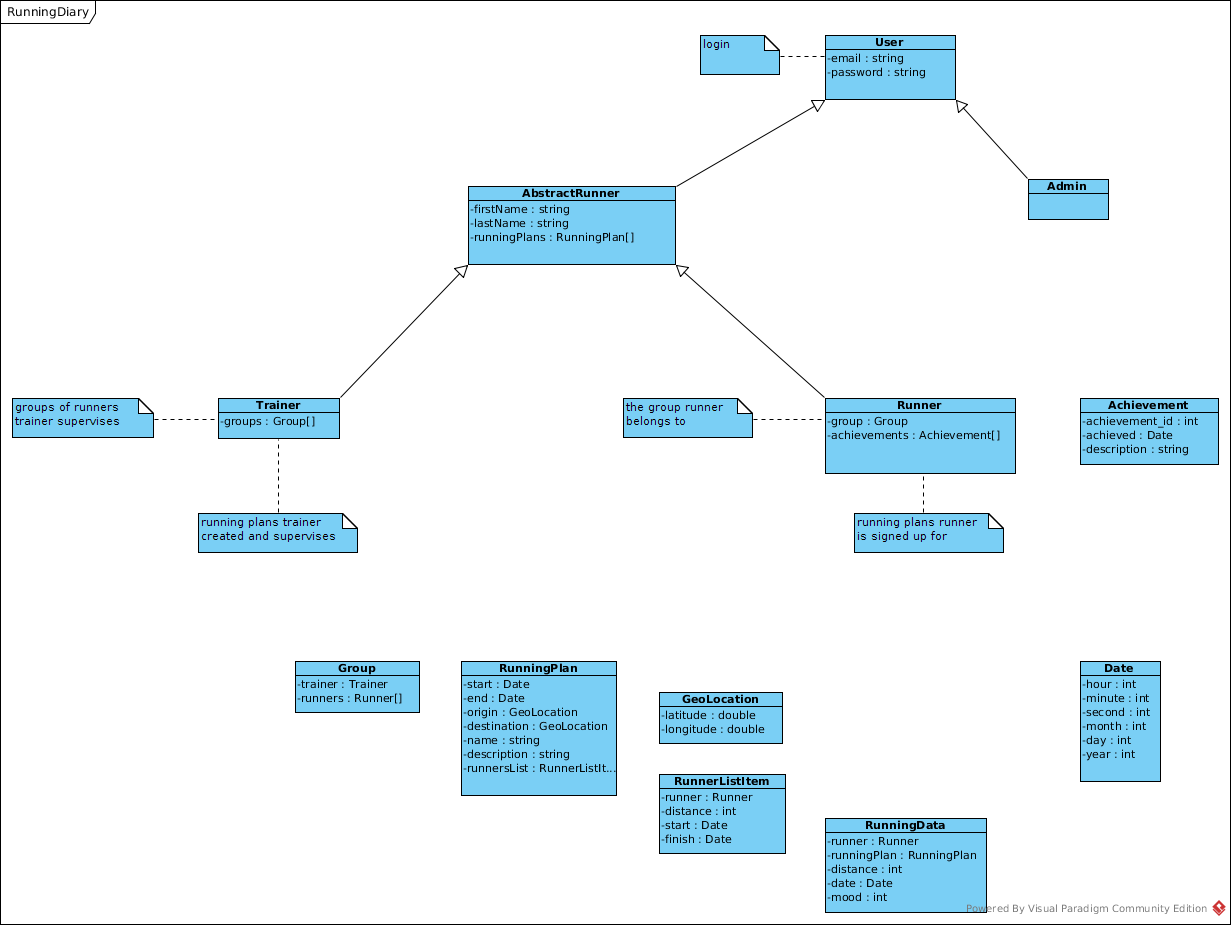
\includegraphics[width=\textwidth]{RunningDiary.png}
\caption{Triedny diagram}
\end{figure}

Triedny diagram ( obr. 2.6 ) je zhmotnením abstrakcie, keď vidíme ake jednotlivé PHP-čkovské triedy dedia spoločné atribúty či metódy od svojich predkov, ako je to aj v prípade AbstractRunnera (resp. Trainera či Runnera) a Admina nakoľko oni všetci podliehajú nutnej podmienke prihlásenia sa do systému v zmysle dodržania dohody o ochrane osobných údajov so súladom s požiadavkami zadávateĺa a disponujú triednymi vlastnosťami email a password.

Perličkou je zdedenie runningPlans v triedach Trainer a Runner kde tento atribút predstavuje úplne iný význam v oboch triedach, čo však vďaka dobre zdokumentovanému návrhu nikdy nebude nesprávne pochopené ani implementačným tímom tretích strán. Konkrétne runningPlans v triede Trainera predstavujú plány, ktoré Trainer vytvoril a spravuje, kdežto v triede Runnera sú to plány, v ktorých je konkrétny bežec prihlásený.

\newpage
\section{Component diagram}
\begin{figure}[H]
\centering
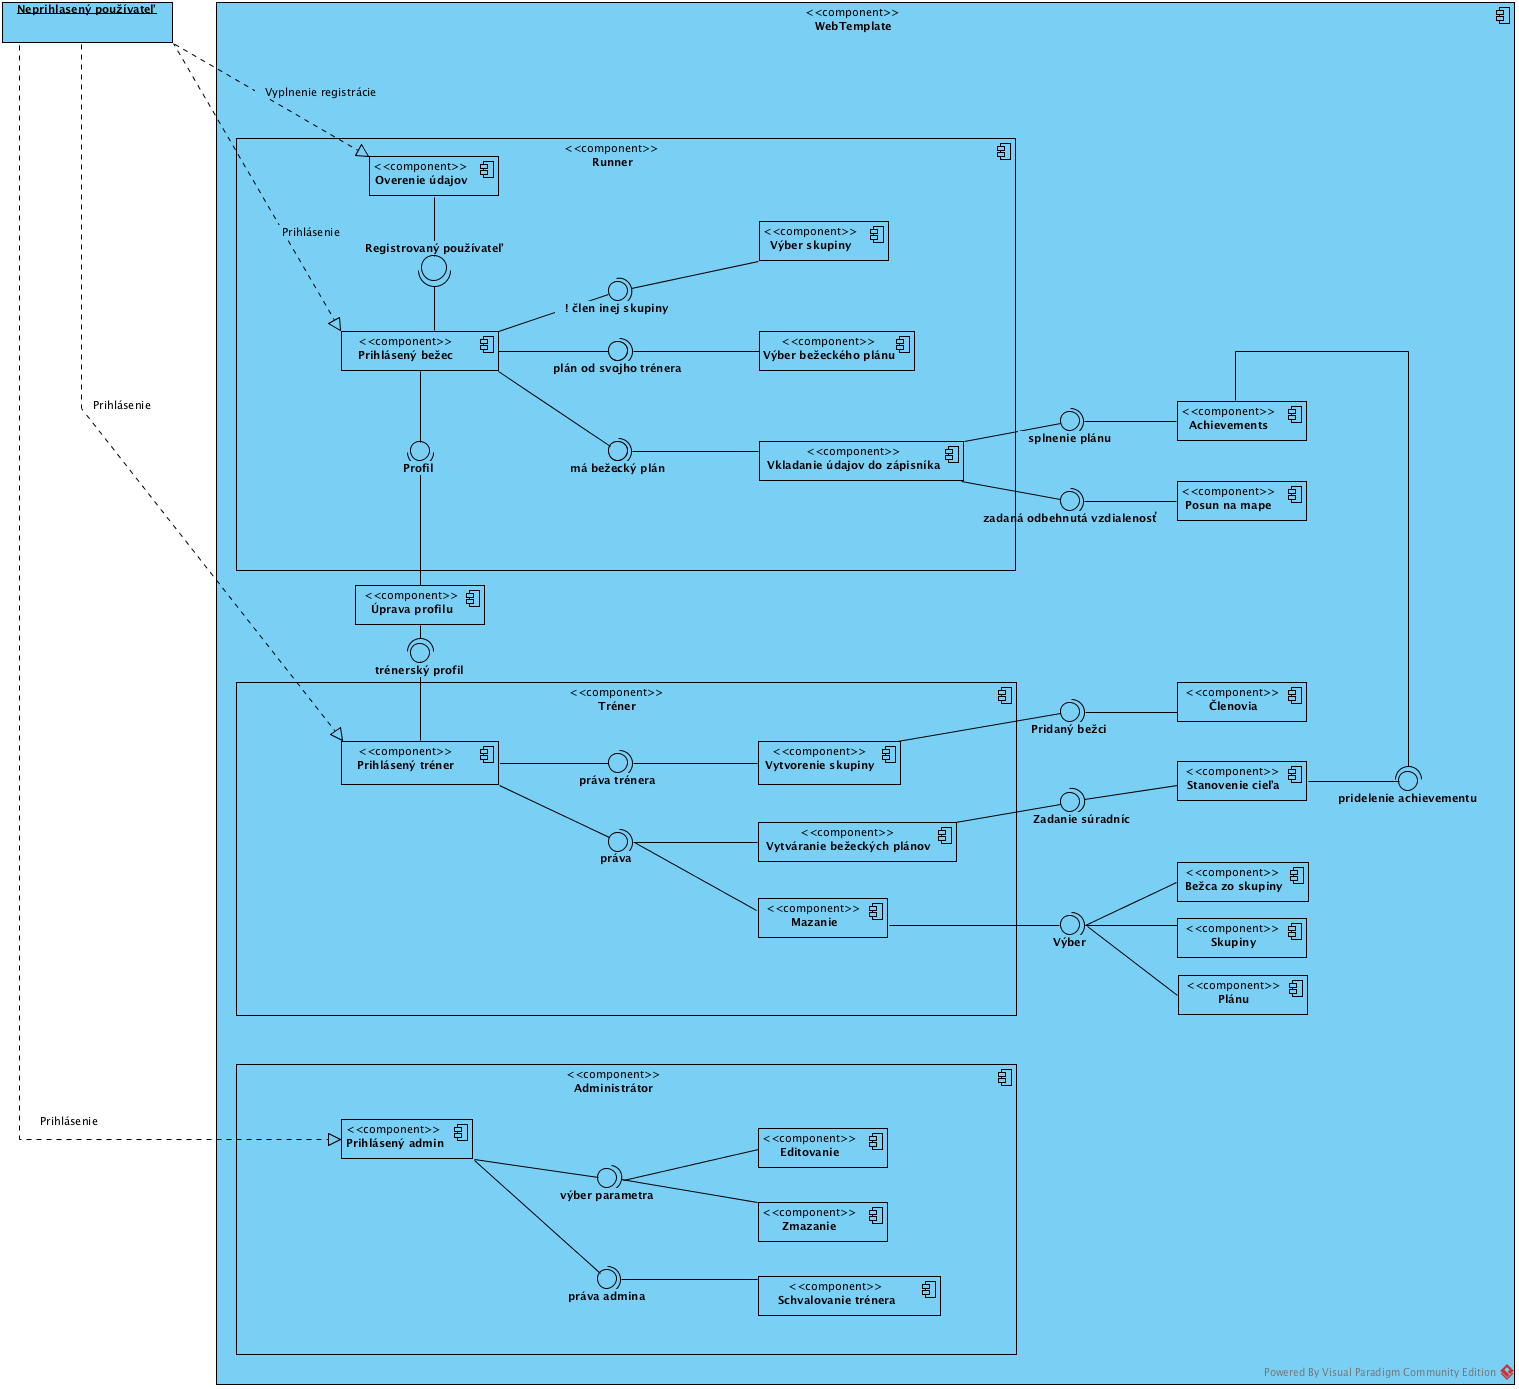
\includegraphics[width=\textwidth]{ComponentDiagram.png}
\caption{Component diagram}
\end{figure}

Component diagram ( obr. 2.7 ) zobrazuje komponenty, ktoré tvoria systém a závislosti medzi nimi. Stručný popis základnej funkcionality kľúčových komponentov:
\begin{itemize}
	\item Component WebTemplate obsahuje celé používateľské rozhranie a dizajn webovej aplikácie. Componet tvoria ďalšie componenty, ktoré môžeme rozdeliť do troch podkategórií do Runner, Tréner, Administrátor a ktoré budú spúšťané podľa výsledku autentifikácie.
	\item Component Úprava profilu umožní Bežcovi alebo Trénorovi upraviť svoj profil, a to napríklad výmenou profilovej fotografie
	\item Component Schvaľovanie trénera umožňuje administrátorovi udeliť obyčajnému bežcovi vyššie právomoci a teda dať mu status Trénera. Tento status mu môže samozrejme aj odobrať.
	\item Component Zmazanie umžňje trénerovi mazať vybrané údaje.
  	\item Component Vkladanie údajov do zápisníka umožňuje Bežcovi vložiť odbehnutú vzdialenosť ktorá sa následne zapíše do databázy a pomocou Componentu Posun na mape Bežec uvidí svoj progres pomocou posunu značky na mape po vyznačenej trase.
	\item Component Mazanie umožňuje Trénerovi mazať dáta podľa zvolených vstupných podmienok. Funkčnosť je podobná ( skoro totožná) s Componentom Zmazanie pre Administrátora.
	\item Component Vytvorenie skupiny umožní Trénoréovi vytvoriť novú skupinu a pridať do nej bežcov.
	\item Component overenie údajov slúži na overenie pravosti údajov zadaných počas registrácie, ak prebehne overenie bez problémov používateľ bude informovaný e-mailom o úspešnej registrácii.
\end{itemize}


\newpage
\chapter{Dátový model}
\begin{figure}[H]
\centering
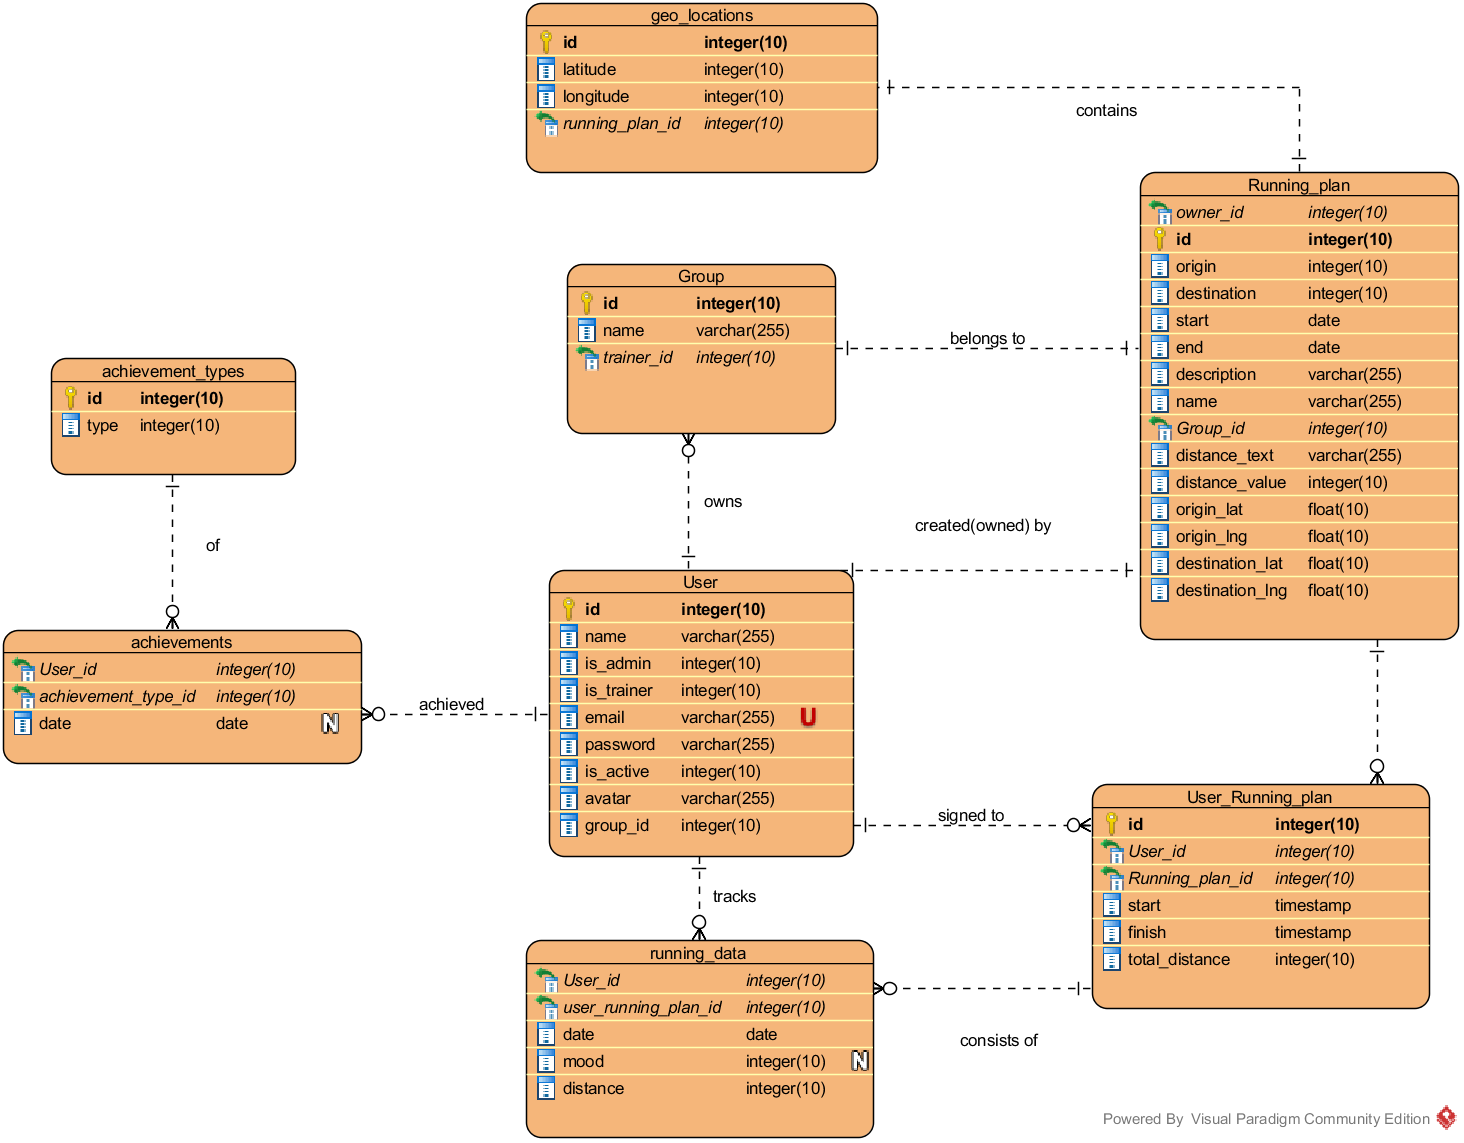
\includegraphics[width=\textwidth]{data_model_updated.png}
\caption{Dátový model}
\end{figure}

Vysvetlivky k diagramu:
\begin{itemize}
\item biele N znamená, že field je nullable
\item červené U znamená, že field je unique
\item zelené šípku označujú cudzie klúče a tučným sú označené primárne klúče
\end{itemize}

\chapter{Testovacie scenáre}
\section{Registrácia}
\begin{itemize}
	\item\begin{itemize}
	\item Vstup: Správne vyplnenie registračnéh formulára.
	\item Výstup: Vytvorenie neaktívneho konta a profilu v databáze, zaslanie email o registrácii.
	\item Stav testovania: Otestované
	\end{itemize}
	
%	\item\begin{itemize}
%	\item Vstup: Potvrdenie požiadavky o regstráciu adminom.
%	\item Výstup: Odoslanie informácie o potvrdení registrácie užívateľovi, aktivácia užívateľovho konta.
%	\item Stav testovania: Treba otestovať
%	\end{itemize}
	
%	\item\begin{itemize}
%	\item Vstup: Odmientutie požiadavky o regstráciu adminom.
%	\item Výstup: Odoslanie informácie o odmietnutí registrácie užívateľovi, vymazanie užívateľovho konta z databázy.
%	\item Stav testovania: Treba otestovať
%	\end{itemize}
	
	\item\begin{itemize}
	\item Vstup: Nesprávne vyplnenie registračného formulára
	\item Výstup: Zobrazenie informácie užívateľovi o zle vyplnených údajoch.
	\item Stav testovania: Otestované
	\end{itemize}
	
	\item\begin{itemize}
	\item Vstup: Snaha o ,,CODE Injection" pri vyplňovaní registračného formulára.
	\item Výstup: Zobrazenie informácie užívateľovi o zle vyplnených údajoch.
	\item Stav testovania: Otestované
	\end{itemize}
\end{itemize}
	

\section{Prihlásenie}
\begin{itemize}
	
	\item\begin{itemize}
	\item Vstup: Správne vyplnené prihlasovacie údaje.
	\item Výstup: Užívateľovi je povolený prístup na stránku.
	\item Stav testovania: Otestované
	\end{itemize}
	
	\item\begin{itemize}
	\item Vstup: Nesprávne vyplnené prihlasovacie údaje.
	\item Výstup: Zobrazenie informácie o zle vyplnených údajoch.
	\item Stav testovania: Otestované
	\end{itemize}
	
	\item\begin{itemize}
	\item Vstup: Snaha o ,,CODE Injection" pri vyplňovaní prihlasovacieho formulára.
	\item Výstup: Zobrazenie informácie užívateľovi o zle vyplnených údajoch.
	\item Stav testovania: Otestované
	\end{itemize}

\end{itemize}
\section{Zmena údajov profilu}
\begin{itemize}

	\item\begin{itemize}
	\item Vstup: Správne vyplnenie nových údajov.
	\item Výstup: Zmena údajov v profile užívateľa.
	\item Stav testovania: Otestované
	\end{itemize}
	
	\item\begin{itemize}
	\item Vstup: Nesprávne vyplnenie nových údajov.
	\item Výstup: Zobrazenie informácie o zle vyplnených údajoch.
	\item Stav testovania: Otestované
	\end{itemize}
	
%	\item\begin{itemize}
%	\item Vstup: Nesprávne zadané heslo pri potvrďovaní zmien v profile.
%	\item Výstup: Zobrazenie informácie o zle vyplnených údajoch.
%	\item Stav testovania: Treba otestovať
%	\end{itemize}
	
	\item\begin{itemize}
	\item Vstup: Snaha o ,,CODE Injection" pri vyplňovaní nových údajov.
	\item Zobrazenie informácie užívateľovi o zle vyplnených údajoch.
	\item Stav testovania: Otestované
	\end{itemize}
	
\end{itemize}
\section{Možnosti bežca po prihlásení}
\begin{itemize}
	\item\begin{itemize}
	\item Vstup: Zobrazenie štatistík.
	\item Výstup: Zobrazenie štatistík prisluchajúcich danému bežcovi a danému bežckému plánu.
	\item Stav testovania: Otestované
	\end{itemize}
	
	\item\begin{itemize}
	\item Vstup: Požiadavka na pridanie do skupiny.
	\item Výstup: Trénerovi danej skupiny príde požiadavka na pridanie bežca do skupiny.
	\item Stav testovania: Otestované
		\begin{itemize}
		\item Vstup: Požiadavka na pridanie do skupiny bola akceptovaná. \\
		Výstup: Bežec je pridaný do skupiny. \\
		Stav testovania: Otestované
		\item Vstup: Požiadavka na pridanie do skupiny bola zamietnutá. \\
		Výstup: Požiadavka zrušená, bežec nepridany do skupiny. \\
		Stav testovania: Otestované
		\end{itemize}
	\end{itemize}
	
	\item\begin{itemize}
	\item Vstup: Opustenie skupiny.
	\item Výstup: Bežec je vyradený zo skupiny.
	\item Stav testovania: Otestované
	\end{itemize}
	
	\item\begin{itemize}
	\item Vstup: Pridanie validných dát do zápisníka.
	\item Výstup: Dáta z behu sa zapíšu do databázy.
	\item Stav testovania: Otestované
	\end{itemize}
	
	\item\begin{itemize}
	\item Vstup: Pridanie nesprávnych dát do zápisníka.
	\item Výstup: Zobrazenie informácie o nesprávne vyplnených dátach.
	\item Stav testovania: Otestované
	\end{itemize}
	
\end{itemize}
\section{Možnosti trénera po prihlásení}
\begin{itemize}
%	\item\begin{itemize}
%	\item Vstup: Zobrazenie štatistík skupiny.
%	\item Výstup: Zobrazenie štatistík prisluchajúcich skupine, ktorej je trénerom.
%	\item Stav testovania: Treba otestovať
%	\end{itemize}
	
	\item\begin{itemize}
	\item Vstup: Vyhodenie bežca zo skupiny.
	\item Výstup: Bežec je vyradený zo skupiny.
	\item Stav testovania: Otestované
	\end{itemize}
	
	\item\begin{itemize}
	\item Vstup: Vytvorenie bežeckého plánu.
	\item Výstup: Bežecký plán sa uloží do databázy.
	\item Stav testovania: Otestované
	\end{itemize}
	
	\item\begin{itemize}
	\item Vstup: Vytvorenie skupiny.
	\item Výstup: Skupina je uložená do databázy.
	\item Stav testovania: Otestované
	\end{itemize}
	
	\item\begin{itemize}
	\item Vstup: Vymazanie skupiny.
	\item Výstup: Skupina je vymazazá z databázy.
	\item Stav testovania: Otestované
	\end{itemize}
	
%	\item\begin{itemize}
%	\item Vstup: Export tabuliek.
%	\item Výstup: Export tabuliek so štatistikami skupiny vo zvolenom formáte.
%	\item Stav testovania: Treba otestovať
%	\end{itemize}
\end{itemize}
\section{Možnosti administrátora po prihlásení}
\begin{itemize}
	\item\begin{itemize}
	\item Vstup: Vybranie užívateľa za trénera.
	\item Výstup: Užívateľ sa stane trénerom.
	\item Stav testovania: Otestované
	\end{itemize}
	
%	\item\begin{itemize}
%	\item Vstup: Úprava údajov užívateľa.
%	\item Výstup: Užívateľovi sa zmenia údaje.
%	\item Stav testovania: Treba otestovať
%	\end{itemize}
	
	\item\begin{itemize}
	\item Vstup: Vymazanie užívateľa.
	\item Výstup: Užívateľské konto je vymazané z databázy.
	\item Stav testovania: Otestované
	\end{itemize}
	
%	\item\begin{itemize}
%	\item Vstup: Vymazanie skupiny.
%	\item Výstup: Všetci bežci patriaci do skupiny obdržia email ,že bola skupina zrušená, tréner tejto skupiny dostane email, že jeho skupina bola vymazaná, všetky bežecké plány suvisiace so skupinou zaniknú.
%	\item Stav testovania: Treba otestovať
%	\end{itemize}
\end{itemize}

\chapter{Používateľská príručka}
\section{Registrácia a prihlásenie}
Pre využitie akejkoľvek funkcionality aplikácie je potrebná registrácia a následné prihásienie. Nový užívateľ po registrácii, dostane potvrdzovací e-mail na e-mail zadaný pri registrácii(ktorý je aj prihlasovacím menom) a musí čakať kým bude jeho účet aktivovaný a až potom sa bude môcť prihlásiť.

\begin{figure}[ht!]
\centering

\includegraphics[width=\textwidth]{menu.png}
\caption{Menu \label{Menu}}
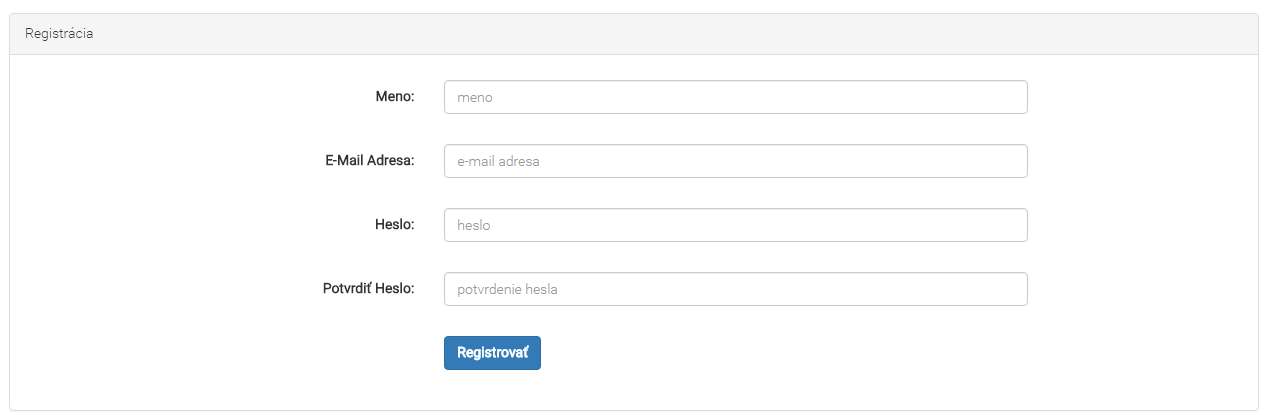
\includegraphics[width=\textwidth]{reg.png}
\caption{Registračný formulár \label{reg}}
\end{figure}

\section{Ovládanie aplikácie}
Aplikácia sa ovláda pomocou horizontálneho menu v hornej časti webového prehliadača:
\begin{itemize}
\item naľavo - tlačidlo Domov, ktoré zobrazí landing page
\item tlačidlá umožňujúce funkcionalitu stránky
\item napravo - profilová fotka a meno užívateľa služiace na prístup k profilu a odhlásenie z aplikácie
\end{itemize}

\begin{figure}[ht!]
\centering

\includegraphics[width=\textwidth]{profil.png}
\caption{Profil používateľa \label{profil}}
\end{figure}
\subsection{Administrácia}

Medzi funkcionality prístupné adminovi patrí:
\begin{itemize}
\item pridávanie trénerov
\item mazanie trénerov
\item aktivovanie užívateľov
\item mazanie užívateľov
\end{itemize}
Prvé dve sú pristupné pomocou prvého tlačidla Tréneri a druhé dve pomocou tlačidla Používatelia. Po kliknutí na jedno z týchto tlačidiel sa zobrazí dropdown s konkrétnou voľbou mazania/aktivovania... Následne sa zobrazí formulár so zoznamom užívateľov/trénerov nad ktorími je možné vykonať danú akciu.

\begin{figure}[H]
\centering

\includegraphics[width=\textwidth]{adminAprove.png}
\caption{Schavaľovanie používateľov \label{adminAprove}}

\end{figure}

\begin{figure}[H]
\centering
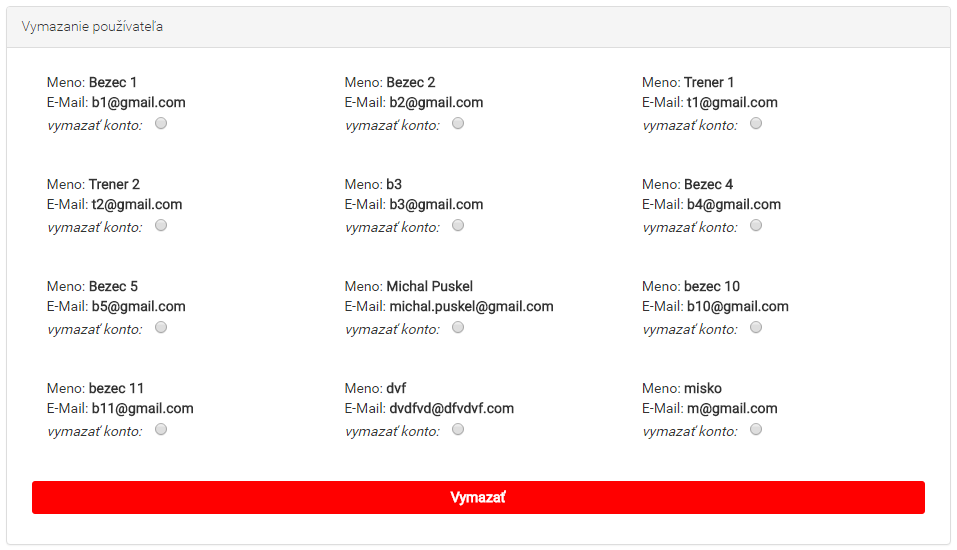
\includegraphics[width=\textwidth]{adminDelete.png}
\caption{Mazanie používateľov \label{adminDelete}}
\end{figure}

\subsection{Tréneri}
Medzi funkcionality prístupné trénerovi patrí:
\begin{itemize}
\item vytvaranie skupín
\item upravovanie skupín
\item mazanie skupín
\item vytváranie bežeckých plánov
\item prezeranie bežeckých plánov
\end{itemize}
Prvé tri funkcie sú prístupné cez tlačidlo Skupiny, ostatné cez tlačidlo Bežecké plány.

\begin{figure}[H]
\centering
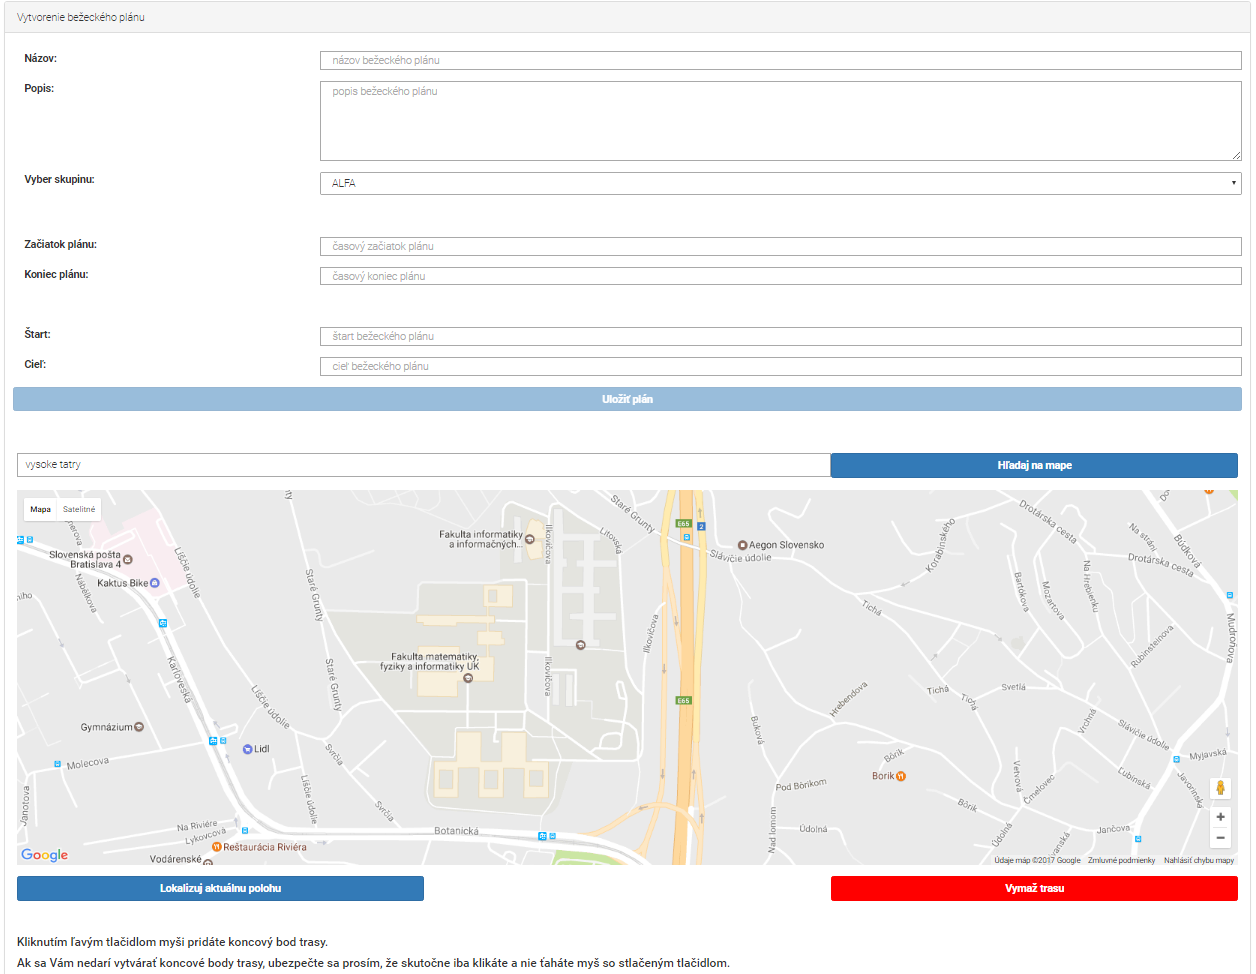
\includegraphics[width=\textwidth]{createRPlan.png}
\caption{Vytvárenie bežeckých plánov \label{createRPlan}}

\end{figure}

\begin{figure}[H]
\centering
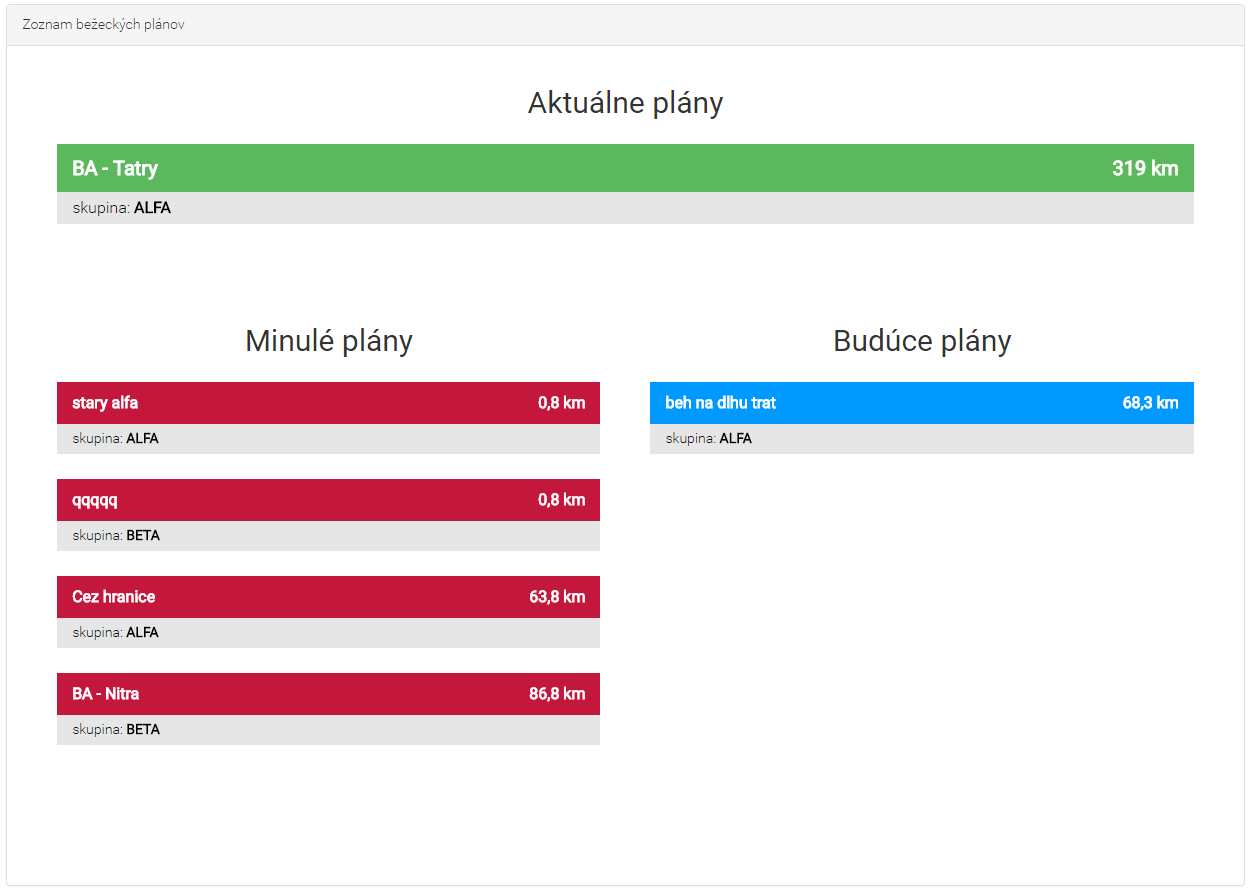
\includegraphics[width=\textwidth]{RPlanList.png}
\caption{Zobrazenie bežeckých plánov \label{RPlanList}}
\end{figure}

\begin{itemize}
\item Po kliknutí na vytvaranie skupín sa trénerovi zobrazí formulár, kde zadá meno skupiny a vyberie si bežcov zo zoznamu, tých bežcov, ktorý nepatria do žiadnej skupiny.
\item Po kliknutí na editovanie skupín sa trénerovi zobrazí formulár, kde si môže vybrať v dropdown menu meno skupiny, ktorú chce editovať. Nasledne po klinutí na tlačidlo edit sa zobrazí formulár, v ktorom je možné zvoliť, ktorý bežci budú zo skupiny vymazaný a ktorý do nej budú pridaný.
\item Po kliknutí na mazanie skupín sa trénerovi zobrazí formulár, kde si môže vybrať skupinu, ktorú chce zmazať
\item Po kliknutí na vytvorenie nového bežeckého plánu sa trénerovi zobrazí formulár, v ktorom tréner vyplní podrobnosti o bežeckom pláne podľa popisov a vyberie trasu na mape pomocou kliknutia na štartový a koncový bod danej trasy. V prípade, že by chcel tréner zmeniť trasu, tak je nutné ju vymazať pomocou tlačidla Vymaž trasu a následne opakovať pôvodný postup.
\item  Po kliknutí na vylistovanie bežeckých plánov sa trénerovi zobrazí formulár, v ktorom sú jednotlivé bežecké plány rozdelené podľa toho či momentálne prebiehajú, či už skončili alebo či ešte len začnú. Po kliknutí na niektorý z týchto plánov sa zobrazí s podrobnosťami o danom pláne a progrese prihásených bežcov. V dolnej časti tohto formulára sa nachádza checkbox, ktorý umožňuje vymazanie plánu.
\end{itemize}
\subsection{Bežci}
Medzi funkcionality prístupné bežcovi patrí:
\begin{itemize}
\item prezeranie bežeckých plánov(súčasťou je aj prihlasovanie a odhlasovanie) - tlačidlo Running plans
\item zápisník - tlačidlo Zápisník
\end{itemize}

\begin{figure}[H]
\centering
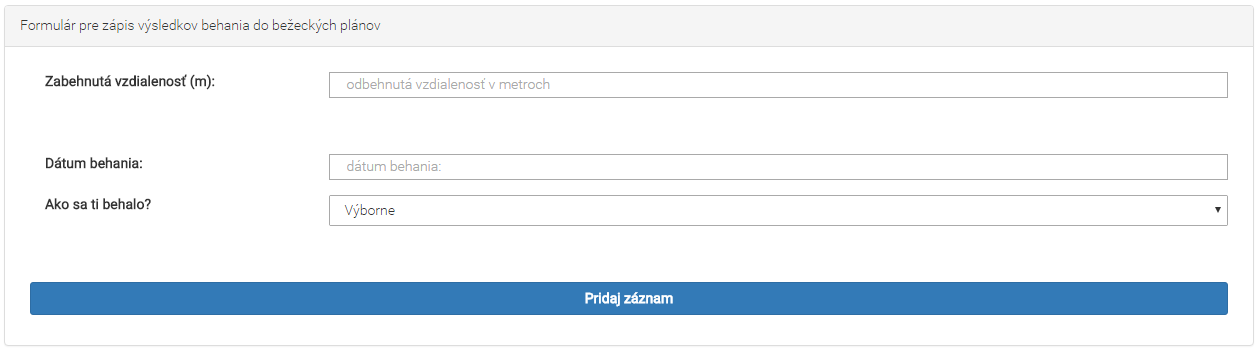
\includegraphics[width=\textwidth]{zapisnik.png}
\caption{Bežecký zápisník \label{zapisnik}}
\end{figure}

\begin{itemize}
\item Po kliknutí na vylistovanie bežeckých plánov sa bežcovi zobrazí zoznam plánov, na ktoré je prihlásený, na ktoré bol prihlásený, ale už skončili a zoznam aktuálnych plánov, na ktoré sa môže prihlásiť. 
\item Po kliknutí na ktorýkoľvek z plánov sa zobrazia informácie o danom pláne, s tým, že v plánoch, na ktoré je bežec prihlásený sa v dolnej časti formulára nachádza tlačidlo pre odhlásenie z plánu a v plánoch, na ktoré sa bežec môže prihlásiť sa nachádza tlačidlo na prihlásenie sa do daného plánu.
\item Po kliknutí na tlačidlo zápisníku a sa zobrazí formulár, ktorý umožňuje zapisovanie bežeckých dát. Tento formulár je potrebné vyplniť podľa popisov jednolivých polí a po kliknutí na tlačidlo Zápis sa tieto dáta zapíšu do všetkých plánov, na ktoré je bežec prihlásený.
\end{itemize}


\chapter{Inštalačná príručka}
Aplikácia sa inštaluje len pridaním celého priečinku do public adresára serveru, na ktorom má fungovať. Tak ako bolo napísané už v špecifikácii, tento server musí podporovať určité knižnice a framework Laravel minimálne vo verzii 5.0.

Pre obnovenie databázy stačí použiť command line príkaz \texttt{php artisan migrate:resfresh --seed}, po zavolaní tohoto príkazu sa bude v databáze nachádzať iba konto admina a všetky ostatné dáta budú vymazané.

\chapter{Záznam z odovzdávania a predvedenia výslednej aplikácie zadávateľovi}
\section{Plán stretnutia}
Stretnutie so zadávateľom pánom Richardom Baloghom sme naplánovali na štvrtok
15.12.2016. Na stretnutie sme naplánovali predvedenie našej aplikácie a jej funkcionality.

\section{Priebeh stretnutia}
Zadávateľa sme v skratke informovali o priebehu našej práce. Určili sme požiadavky ktoré
boli splnené, ktoré zatiaľ neboli splnené, prečo sa tak stalo a či budú splnené dodatočne.
Predviedli sme aplikáciu a jej funkcionalitu pre rôznych užívateľov (bežec, tréner a administrátor).

\section{Pripomienky}
Zadávateľ nemal žiadne pripomienky, s tým, že sme sa dohodli, že ostávajúce časti aplikácie budú hotové do Vianoc a že pre účely testovania by chcel, aby sme dali aplikáciu na nejaký server, lebo inštalácia u neho trvá veľmi dlho.

\section{Implementácia pripomienok}
Aplikácia bola pre testovacie účely sprístupnená na našej webstránke. Všetky funkcie boli dokončené v trochu neskoršom dátume, kvôli vianočným sviatkom a povinnostiam členov týmu.

\chapter{Zhodnotenie}
\section{Spokojnosť s výsledným dielom a problémy počas vývoja}
Všetci členovia tímu sú s výsledným dielom spokojný. Podarilo sa nám implementovať
všetky požiadavky zadávateľa v dohodnutých termínoch.

Počas vývoja sa vyskytlo niekoľko problémov, ktoré sa však podarilo úspešne vyriešiť.
Jedným z problémov bola neskúsenosť členov tímu s frameworkom Laravel a prácou s GoogleMaps API, kde boli problémy napríklad s hľadaním pozícií na trase a s granularitou samotnej trasy. Tieto problémy sa podarilo pomocou materiálov nájdených na internete a tímovej spolupráce vyriešiť.

\section{Zmeny do ďalších verzií}
Cieľom, na ktorom sme sa dohodli so zadávateľom bolo, urobiť aplikáciu, ktorá robí len pár vecí, ale robí ich poriadne. Tým pádom ešte stále ostáva priestor na vylepšenia a ďaľšie funkcionality, ktoré sú popísané v sekcii 2.4 Budúca verzia systému, ako napríklad prihlasovanie pomocou Google účtu alebo Facebooku, alebo nástenka s oznamami.

\section{Odlišnosti od pôvodného plánu}
Počas implementácie prišlo k niekoľkým zmenám oproti plánu:

\begin{itemize}
\item Zmeny v dátovom modely, kvôli použitiu Laravelu, s ktorým sa v čase tvorby modelu plne nerátalo.
\item Umoženenie vytvárania viacerých skupín trénerom(pôvodne sa rátalo len s jednou skupinou).
\item Uprávy niektorých fukcií do podoby v akej sú popísané v tomto dokumente, kvôli nepochopenia zámeru zadávateľa
\end{itemize}

\section{Tímová práca, rozdelenie úloh a komunikácia}
O všetkých problémoch sa diskutovalo na skupinových stretnutiach. Na väčšinu komunikácie sa využívala facebooková konverzácia, pomocou ktorej sme si aj posielali niektoré dokumenty.
Všetky materiály sme ukladali do našeho repozitáru na GitHube.

Úlohy sme si rozdelovali podľa momentálnych časových možností a skúseností s konkrétnym problémom, ktorý sme riešili. Kedže Tomáš má skúsenosti s dizajnom, tak si on zobral na starosti vytvorenie loga a užívateľského prostredia aplikácie. Nakoľko Michal viedol našu prácu na implementácii, tak mal aj na starosti prácu Google mapou, ktorá bola nakomplexnejšou častou samotnej aplikácie. Martin sa postaral o vytvorenie funkcionalít súvisiacich s databázou a Jaro vytvoril zápisník a testovacie scenáre, ktoré boli využité pri kontrole funcionalít výslednej aplikácie.

S tímovou spoluprácou boli všetci členovia spokojný, keďže na rozdelení úloh aj ostatných
záležitostiach týkajúcich sa spolupráce sme sa vždy dohodli rýchlo a bez problémov. Pokiaľ
mal niekto so svojou časťou projektu akékoľvek problémy na tímovom stretnutí sa tieto
problémy prediskutovali a vyriešili. 

\bigbreak
\noindent Pár slov od každého člena týmu:
\begin{itemize}
\item Michal Puškel: Práca na projekte sa mi veľmi páčila, som veľmi spokojný so všetkými členmi tímu, každý si vždy niečo našiel, kde vedel pomôcť a nikoho do toho netrebalo nútiť, nikto neovláda všetko, ale my sme boli dobre zložení a vzájomne sme sa dopĺňali. Vytvorili sme myslím v skutku užitočnú web aplikáciu, do ktorej sme vložili naozaj veľa lásky, teda veríme, že aj koncoví užívatelia s ňou budú spokojní, ale toto overí iba čas. Dbali sme aj na pohodlné UX ako aj veľkú bezpečnosť, aby bola aplikácia pripravená do reálneho sveta a nie iba tak, že za to chceme známku, sú tam tie najrôznešie kontroly či už zlých používateľských vstupov ale aj ochrana proti neoprávnenému prístupu k údajom resp. editáci a mazaniu čo je ešte kľúčovejšie. Veľmi dlho som už počúval o Laraveli dobré veci... ale som bol stále lenivý ho ošahať, čo sa mi už konečne vďaka tomuto projektu podarilo, takže určite to bol rozumne strávený čas a myslím, že všetci sme sa naučili niečo, čo môžme aj použiť možno v budúcnosti či už na pracovné alebo osobné účely.

V neposlednom rade veľmi ďakujeme všetci Tomášovi Slámovi, hlavne za to že nás svojou húževnatosťou nielen ale aj spoznávať nové technológie dokopal k Laravelu a v tom najkritickejšom čase keď, sme ešte ostatní neboli rozbehnutí, tak Tomáš nielen, že nás rozbehol, ale položil výborné základy celého Laravelového projektu, kompletne vyriešil administráciu užívateľov a všetko čo s ňou bolo spojené, no nezastavil sa! Svoje kvality nám dokazoval aj naďalej deň čo deň, častokrát aj noc čo noc, lebo tento projekt si skutočne vyžadoval vypotiť nejednu kvapku krvi, a pomohol ešte pri riešení mnohých programátorských problémov a jeho zručnosti serverového administrátora boli tým "vitálnym" pojivom, bez ktorého by sa celý projekt rozsypal ako domček z kariet.


\item Tomáš Sláma: Nakoľko už od vyberania členov tímu sme vedeli rozdelenie svojich úloh a uvedomovali si
schopnosti a prednosti každého člena, spolupráca a komunikácia bola na vynikajúcej úrovni.
Ani raz nenastala situácia že by niektorý z členov nesplnil svoje úlohy, prípadne prestal komunikovať.
Každý sa pokúšal robiť aj viac než mal v týždennom pláne a pokúšal sa pomôcť ostatným členom tímu,
aby práce na aplikácii napredovali. 
Martinovi Heinzovi sa musíme poďakovať za dobre navrhnutú databázu, ktorú nebolo počas celého vývoja skoro vôbec 
upravovať, databázové controllery a migrácie.
Michal Puškel skvelo vyriešil mapy, prepočítavanie trasy a posúvanie avatarov po mape. Spolu s Jaslavom Fúskom vyriešili
zapisovanie údajov do zápisníka, bežecké plány a ich intuitívnosť a jednoduchosť. Nemamalé zásluhy patria každému členovi tímu 
na debugovaní a úpravách UI, aby bolo čisté a prehľadné aj pre deti.

Spoluprácu hodnotím veľmi pozitívne a určite by som šiel do ďalšieho projektu v rovnakom zložení.
\item Jaro Fúska: Z môjho pohľadu hodnotím prácu v tíme ako dobrú skúsenosť. Každý odviedol svoj kus práce a nevznikali takmer žiadne nedorozumenia a zásahy do kompetencií členov tímu čo býva najväčším problémom pri skupinových projektoch a čoho som sa aj pred začatím projektu obával. Ako najpozitívnejšie a  zároveň aj najnegatívnejšie hodnotím to, že sa jednalo o webovú aplikáciu kedže mám k tomuto typu aplikácií mierny odpor. Som rád, že som bol donútený pracovať s týmto typom technológie, pričom sme si ako projektový spolupracovníci pomáhali a vždy sa bolo na koho obrátiť. Zároveň však musím dodať, že moje sympatie k tejto časti informatického sveta sa vážnym spôsobom nezmenili. Myslím, že projekt dopadol dobre a aplikácia je v tejto podobe plne využiteľná. Vyskúšali sme si nové technológie a postupy a vytvorili sme niečo čo môžme s hrdosťou spomenúť pri budúcich pohovoroch do práce.


\item Martin Heinz: Prácu celého týmu hodnotím pozitívne, myslím, že každý si plnil úlohy, ktoré sme si na začiatku rozdelili a mám pocit, že sa všetci snažili pomôcť s tým čo bolo práve potrebné spraviť ak to aspoň trochu dovolovali naše časové možnosti počas tohoto náročného semestra.
Čo sa týka projektu ako takého, tak určite tu boli určité problémy, s ktorými sme zápasili, ale tomu sa nedá pri takomto projekte vyhnúť, ale v konečnom dôsledku sme boli schopný sa cez všetko bez väčších problémov dostať.

\end{itemize}

\section{Záver}
Táto správa opisuje vývoj systému Športový klub(bežecký zápisník) od prvých návrhov až po
kompletnú implementáciu s dokumentáciou. Už od začiatku sme sa snažili, aby naše výsledné
dielo zodpovedalo požiadavkám zadávateľa a aby bolo v budúcnosti dobre využiteľné.
Myslíme, že tento cieľ sa podarilo splniť. Práca na tomto projekte nám dala presnú predstavu
o práci v kolektíve, rozdelovaní úloh a dodržiavaní stanovevých termínov. Preto tento projekt
hodnotíme ako cennú skúsenosť a veríme, že nám táto skúsenosť pomôže pri právi na ďaľších projektoch, na ktorých budeme v budúcnosti pracovať.































\end{document} 